\documentclass[10pt,landscape]{article}
\usepackage{multicol}
\usepackage{calc}
\usepackage{ifthen}
\usepackage[landscape]{geometry}
\usepackage{graphicx}
\usepackage{amsmath, amssymb, amsthm}
\usepackage{latexsym, marvosym}
\usepackage{pifont}
\usepackage{lscape}
\usepackage{graphicx}
\usepackage{array}
\usepackage{booktabs}
\usepackage[bottom]{footmisc}
\usepackage{tikz}
\usetikzlibrary{shapes}
\usepackage{pdfpages}
\usepackage{wrapfig}
\usepackage{enumitem}
\setlist[description]{leftmargin=0pt}
\usepackage{xfrac}
\usepackage[pdftex,
            pdfauthor={William Chen},
            pdftitle={Probability Cheatsheet},
            pdfsubject={A cheatsheet pdf and reference guide originally made for Stat 110, Harvard's Introduction to Probability course. Formulas and equations for your statistics class.},
            pdfkeywords={probability} {statistics} {cheatsheet} {pdf} {cheat} {sheet} {formulas} {equations}
            ]{hyperref}
\usepackage{relsize}
\usepackage{rotating}

 \newcommand\independent{\protect\mathpalette{\protect\independenT}{\perp}}
    \def\independenT#1#2{\mathrel{\setbox0\hbox{$#1#2$}%
    \copy0\kern-\wd0\mkern4mu\box0}} 
            
\newcommand{\noin}{\noindent}    
\newcommand{\logit}{\textrm{logit}} 
\newcommand{\var}{\textrm{Var}}
\newcommand{\cov}{\textrm{Cov}} 
\newcommand{\corr}{\textrm{Corr}} 
\newcommand{\N}{\mathcal{N}}
\newcommand{\Bern}{\textrm{Bern}}
\newcommand{\Bin}{\textrm{Bin}}
\newcommand{\Beta}{\textrm{Beta}}
\newcommand{\Gam}{\textrm{Gamma}}
\newcommand{\Expo}{\textrm{Expo}}
\newcommand{\Pois}{\textrm{Pois}}
\newcommand{\Unif}{\textrm{Unif}}
\newcommand{\Geom}{\textrm{Geom}}
\newcommand{\NBin}{\textrm{NBin}}
\newcommand{\Hypergeometric}{\textrm{HGeom}}
\newcommand{\HGeom}{\textrm{HGeom}}
\newcommand{\Mult}{\textrm{Mult}}

\geometry{top=.4in,left=.2in,right=.2in,bottom=.4in}

\pagestyle{empty}
\makeatletter
\renewcommand{\section}{\@startsection{section}{1}{0mm}%
                                {-1ex plus -.5ex minus -.2ex}%
                                {0.5ex plus .2ex}%x
                                {\normalfont\large\bfseries}}
\renewcommand{\subsection}{\@startsection{subsection}{2}{0mm}%
                                {-1explus -.5ex minus -.2ex}%
                                {0.5ex plus .2ex}%
                                {\normalfont\normalsize\bfseries}}
\renewcommand{\subsubsection}{\@startsection{subsubsection}{3}{0mm}%
                                {-1ex plus -.5ex minus -.2ex}%
                                {1ex plus .2ex}%
                                {\normalfont\small\bfseries}}
\makeatother

\setcounter{secnumdepth}{0}

\setlength{\parindent}{0pt}
\setlength{\parskip}{0pt plus 0.5ex}

% -----------------------------------------------------------------------

\usepackage{titlesec}

\titleformat{\section}
{\color{blue}\normalfont\large\bfseries}
{\color{blue}\thesection}{1em}{}
\titleformat{\subsection}
{\color{cyan}\normalfont\normalsize\bfseries}
{\color{cyan}\thesection}{1em}{}
% Comment out the above 5 lines for black and white

\begin{document}

\raggedright
\footnotesize
\begin{multicols*}{3}

% multicol parameters
% These lengths are set only within the two main columns
%\setlength{\columnseprule}{0.25pt}
\setlength{\premulticols}{1pt}
\setlength{\postmulticols}{1pt}
\setlength{\multicolsep}{1pt}
\setlength{\columnsep}{2pt}

%%%%%%%%%%%%%%%%%%%%%%%%%%%%%%%%%%%%
%%% TITLE
%%%%%%%%%%%%%%%%%%%%%%%%%%%%%%%%%%%%

\begin{center}
    {\color{blue} \Large{\textbf{Probability Cheatsheet v2.0}}} \\
   % {\Large{\textbf{Probability Cheatsheet}}} \\
    % comment out line with \color{blue} and uncomment above line for b&w
\end{center}

%%%%%%%%%%%%%%%%%%%%%%%%%%%%%%%%%%%%
%%% ATTRIBUTIONS
%%%%%%%%%%%%%%%%%%%%%%%%%%%%%%%%%%%%

\scriptsize

Compiled by William Chen (\url{http://wzchen.com}) and Joe Blitzstein, with contributions from Sebastian Chiu, Yuan Jiang, Yuqi Hou, and Jessy Hwang. Material based on Joe Blitzstein's (\texttt{\href{http://twitter.com/stat110}{@stat110}}) lectures (\url{http://stat110.net}) and Blitzstein/Hwang's Introduction to Probability textbook (\url{http://bit.ly/introprobability}). Licensed under \texttt{\href{http://creativecommons.org/licenses/by-nc-sa/4.0/}{CC BY-NC-SA 4.0}}. Please share comments, suggestions, and errors at \url{http://github.com/wzchen/probability_cheatsheet}.

\begin{center}
    Last Updated \today
\end{center}

% Cheatsheet format from
% http://www.stdout.org/$\sim$winston/latex/

%%%%%%%%%%%%%%%%%%%%%%%%%%%%%%%%%%%%
%%% BEGIN CHEATSHEET
%%%%%%%%%%%%%%%%%%%%%%%%%%%%%%%%%%%%




Cards in a deck: 52.  \hfill \\
Ace, 2, 3, 4, 5, 6, 7, 8, 9, 10, Jack, Queen, King \hfill \\

\section{Problem solving tips}
Recognize complicated versions of simple formulas.  E.g. $P(A \mid B) = P(A \cap B)/P(B)$ with an $A$ or $B$ like $(A \cup B^c)$ \hfill \\
\textbf{At least} is a trigger for 1 $-$ probability of all items.  E.g. probability you will roll at least one 6 in 3 die rolls $= 1 - P(\mbox{no 6s rolled}) = 1 - (5/6)^3$. 


\section{Probability Formulas}
\smallskip \hrule height 2pt \smallskip

\begin{description}
	\item[Misc.] 
		\begin{align*}
		\Phi &= \Omega^c   \mbox{\tiny{(Lecture 4)}}  \\
		\cap E_i &= (\cup E_i^c)^c       \mbox{\tiny{(Lecture 4)}}  \\
		%\[ A \cup A^{c} =U  \]
		%\[ A \cap A^{c} =\Omega  \]
		A \cup A^{c} &= \Phi  
		\end{align*}

		
		\textbf{DeMorgan's laws}, pg 26:  You can distribute/factor a complement if you switch the $\cup$ or $\cap$ \\
		\[  (A \cup B)^c = A^c \cap B^c  \]
		\begin{center} \tiny{so $P((A \cup B)^c) = P(A^c \cap B^c)$}   \end{center}  
		\[   (A \cap B)^c = A^c \cup B^c  \]
		
		Goal: you have one complement in your "and" space and don't want it.  $A \cap B^c = A -(A \cap B)$  Use Venn diagrams to see.   (in pg 37 proof)
		
		What about $A \cup B^c$?  ???
		\hfill \\
		\begin{align*}
		P(A \cap B) + P(A^c \cap B) &= P(B)  \mbox{   \tiny{(in prob 2.4.5 pg 37)}}   \\
		P(A \cup B) + P(A^c \cup B) &= 1  \mbox{   \tiny{(logically b/c $P(A) + P(A^c) = 1$}}  \\
		\end{align*}
		
\end{description}

%%%%%%%%%%%%%%%%%%%%%%%%%%%%%%%
\subsection{Mutually exclusive and/or exhaustive}
    \begin{description}
    
    	\item[Mutually exclusive] ${E_1}, {E_2}$ are \textit{mutually exclusive} if 
        		$P({E_1} \cup {E_2} \cup {E_3} \cup ...) = P({E_1}) + P({E_2}) + P({E_3}) + ...$   \\
		%\begin{flushright} \tiny{(Lec 2, L\&M 2.3)} \end{flushright}
		{ \tiny (Lec 2, L\&M 2.3)}.   \\
		Note that then $ P(E_i \cap E_j) = 0 $
    
    
    	\item[Mutually exclusive and exhaustive] 
	\[ \mbox{For } E_1, E_2, \dots:  \]
	\[ E_i \cap E_j = \Phi \mbox{, } P(E_i \cap E_j) = 0 \mbox{, and } \Omega = E_1 \cup E_2 \cup \dots \]
	\[ \mbox{ Mutually exclusive + exhaustive = partition } \]
    \end{description}

%%%%%%%%%%%%%%%%%%%%%%%%%    
\subsection{The fundamental laws of set algebra} {\tiny (Wikipedia)}

	\textbf{Commutative Laws}
		\begin{align*}
			A \cup B = B \cup A   \\
			A \cap B = B \cap A   \\
		\end{align*}
     \textbf{Associative Laws}
		\begin{align*}
			(A \cup B) \cup C = A \cup (B \cup C) \\
			(A \cap B) \cap C = A \cap (B \cap C) \\
		\end{align*}
	\textbf{Distributive laws}
		\[ A \cup (B \cap C) = (A \cup B) \cap (A \cup C)   \]
		\[ A \cap (B \cup C) = (A \cap B) \cup (A \cap C) \]
    
%%%%%%%%%%%%%%%%%%%%%%%%%%%%			
	
\subsection{Basic probability formulae}
           \begin{gather*} 
        		\Omega = E \cup E^c \\
        		E \cap E^c = \Phi \\
      		\mbox{ so }  P(E^c) + P(E) = P(\Omega) = 1, or P(E^c) = 1-P(E) \\
        		\mbox{ and} P(D)  \leq 1 \mbox{, since all probabilities are non-negative} \\
           E \cup F = E \cup (E^c \cap F)  \\
            \mbox{and E and $E^c$ are disjoint, so you can break them apart} \\            
           P(E \cup F) = P(E) + P(E^c) \cap F \\
           \mbox{so } P(E \cup F) + P(E \cap F) =  \\ P(E) + P(E^c \cap F) + P(E \cap F) = P(E) + P(F) \\
           \mbox{restated: } P(E \cup F) + P(E \cap F) = P(E) + P(F) \\
           \end{gather*}  
    
\begin{description}
\item[Law of total probability] See Lec2, L\&M 2.3 \newline
For events E, F of a partition, you can build F or P(F) from the overlaps of the events E with P.
	\[ F = U_i(F \cap E_i)  \]
	\[ P(F) = \sum_{n=1} P(F \cap E_i) \]
Special case: If $E_i$ is the \textit{i}th outcome in a countable $\Omega$, $F \cap E_i = Ei$ 
or $F \cap E_i = \Phi$ and $P(F) = \sum_{i \in F} P(E_i)$.  \hfill \\
\hfill \\
Example {\tiny my 1st stat lecture}:  P(3 face cards in a row).  Note: 40 of the 52 cards in a deck are non-face cards.  Let $C_i$ = the event corresponding to drawing a non-face card on draw $i$.  Then 
	\begin{align*}
		P(C_1 \cap C_2 \cap C_3) &= P(C1)  \cdot P(C_2 \mid C_1) \cdot P(C_3 \mid C_2 \cap C_1) \\
			&= (40/52) \cdot (39/51) \cdot (38/50) 
	\end{align*} 
	\hfill \\
  \hfill \\


\item[The inclusion and exclusion formula] (The overlapping tiles sum)
If you want to get the $\cup$ of some events, sum all the areas, subtract out the singly over lapping bits, add back the tripply overlapping bits, subtract off the quadruply overlapping bits, etc.  Go as far as the number of Es you have. 
All cups on the left side and caps on the right. 
	\[\mbox{2 items: } P(D \cup E) = P(D) + P(E) - P(D \cap E) \]
	\begin{align*}
	\mbox{3 items: }   
	P(C \cup D \cup E) = P(C) + P(D) + P(E) \\
	\quad - P(C \cap D) - P(D \cap E) - P(E \cap C) \\
	\quad + P(C \cap D \cap E) \\
	\end{align*}

\item[Review ways of breaking apart $\cup$ \& and $\cap$] \hfill \\

 You can relate cap and cup {\tiny by Theorem 2.3.6 (pg 28)}:
$P(A \cup B) = P(A) + P(B) - P(A \cup B)$, which can be re-arranged.  \hfill \\
\hfill \\
$\cup$ covers two areas.  If they are independent you can separate them with pluses.  If you know about their $\cap$ you can deduce their $\cup$.  \hfill \\
\hfill \\
$\cap$ is the

\end{description}

%%%%%%%%%%%%%%%%%%%%%
\section{Conditional probability}
\smallskip \hrule height 2pt \smallskip

\begin{description}
\item[Relating conditional probability \& intersection]     L\&M pg 34, L5. \hfill \\
If P(B) \textgreater 0:
	\begin{align*}
		P(A \mid B) = \frac{ P(A \cap B) }{ P(B) }   \hfill \\
	\end{align*}
How to remember if you got the $\mid$ and $\cap$ in the right order: visualize the and inside the circle.

\hfill \\
This gives you a way to relate intersections and conditional probabilities:
$P(A \cap B) = P(A \mid B)P(B)$  (pg. 34)

\item[Some more tricks]
	%\begin{align*}
	Recognize the relation between $A \cup B$  and $A \cap B$ even if there is something like $(A \cup B) \cap (A \cup B)^c$.  You can pull the c inside and write the $P(A) + P(B)$ type statement.
	%\end{align*}
	
\item[A+B and A-B without P involved]
Generally avoid adding sets.  Adding and subtracting probability of sets is great though. \hfill \\
With that warning, The definition of $A-B$ is $A \cap B^c$.  Note that $P(A-B) \neq P(A) - P(B)$.  Wikipedia uses \textbackslash  for $-$ in sets. \hfill \\ 
E suggests always avoiding + when doing math of sets.  It's fine to have + when probability is involved, but adding sets doesn't make a lot of sense.  You could call $\cup$ addition, but that is confusing.  
\end{description}

\subsection{The chain rule}
If you don't want to use intersections, you can use only conditional probabilities to calculate an intersection.  {\tiny L\&M pg 43.}
If $P(E_1 \cap E_2 \cap \dots \cap E_n) > 0$, \hfill \\
$P(E_1 \cap E_2 \cap \dots \cap E_n)$  \hfill \\ 
$= P(E_1)P(E_2 \mid E1)P(E_3 \mid E1 \cap E2) \dots P(E_n \mid E_1 \cap E_2 \cap \dots \cap E_n)$.
 Note you could put $E_1, E_2, \dots$ in any order you want (commutative rule).  Also note that there is no cool rul for $P(A \cup B \cup C)$ \hfill \\ 
 \hfill \\
Review: if you want to break apart unions, you think of the tiles overlapping and subtracting/adding sections intersections back.  If you want to break apart intersections, you can use the chain rule to break it into conditional probabilities.  
 \hfill \\
 
 \subsection{Law of total probability} {\tiny Lecture 5, L\&M pg 43}   \hfill \\
 If you have mutually exclusive and exhaustive events $H_i$, and $i = 1, \dots k$.  Mutually exclusive \& exhaustive means $\sum_{i=1}^k P(H_i) = 1$.  Note also $H_i \cap H_j = \Phi$, $P(H_i \cap H_j) = 0$  
 Since $D = (D \cap H_1) \cup (D \cap H_2) \cup \dots \cup  (D \cap H_k)$
	\begin{align*}
 		P(D) = \sum_{j=1}^k P(D \mid H_j) P(H_j) 
  	\end{align*}
We are summing across outcomes, and weighting the sums by the likelyhood of the sub-outcomes.
 
 \subsection{Bayes' formula} {\tiny L\&M p48, Lecture 5}
 Assume $H_i$, $i = 1, \dots, k$ as above (mutually exclusive and exhaustive), and $D$ with $P(D) > 0$.
 	\begin{align*}
		P(H_j \mid D) = \frac{P(H_j \cap D)}{P(D)} = \frac{P(D \mid H_j) P(H_j) }{\sum_{i=1}^k P(D \mid H_j) P(H_j) }
	\end{align*}
$P(\mbox{have antigen A} \mid \mbox{have antigen B}) = P(AB)/(P(B) + P(AB)) $  \hfill \\
 \hfill \\
 
 Example {\tiny (J's Lecture 1)}.  Coin $C_1$ has probability $1/4$ of giving heads.  Coin $C_2$ has probability $1/2$ of giving heads.  What is $P(C_1 \mid H)$?  Bayes theorem.   
 	\begin{align*}
	P(C_1 \mid H) &= P(C_1 \cap H)/P(H) \\
		&\mbox{use } P(C_1 \cap H) = P(H \mid C_1) \cdot P(C_1) \\
		&\mbox{use } P(H) = P(H \mid C_1) \cdot P(C_1) + P(H \mid C_2) \cdot P(C_2) \\
			& = \frac{P(H \mid C_1) \cdot P(C_1)}{P(H \mid C_1) \cdot P(C_1) + P(H \mid C_2) \cdot P(C_2)} \\
			&= \frac{(1/4)\cdot (1/2)}{(1/4)\cdot (1/2) + (3/4)\cdot (1/2) } = \frac{1}{4}\\
	\end{align*}
If you get heads again, what is your probability of coin 1? Call your $P(C_1)$ from above $P^*(C_1)$.  Now $P(H_2)$ (probability of a 2nd heads) is:
	\begin{align*}
	P(C_1 \mid H_2) &= P(C_1 \cap H_2)/P(H_2) \\
		&\mbox{use } P(C_1 \cap H_2) = P(H_2 \mid C_1) \cdot P^*(C_1) \\
		&\mbox{use } P(H_2) = P(H_2 \mid C_1) \cdot P^*(C_1) + P(H_2 \mid C_2) \cdot P^*(C_2) \\
			& = \frac{P(H_2 \mid C_1) \cdot P^*(C_1)}{P(H_2 \mid C_1) \cdot P^*(C_1) + P(H_2 \mid C_2) \cdot P^*(C_2)} \\
			&= \frac{(1/4)\cdot (1/4)}{(1/4)\cdot (1/4) + (3/4)\cdot (3/2) } = \frac{1}{10}\\
	\end{align*}
We could have done it without Bayes: Instead use $P(HH)$ which is P(two heads).  
	\begin{align*}
	P(C_1 \mid HH) &= P(C_1 \cap HH)/P(HH) \\
		&\mbox{use } P(C_1 \cap HH) = P(HH \mid C_1) \cdot P(C_1) \\
		&\mbox{use } P(HH) = P(HH \mid C_1) \cdot P(C_1) + P(HH \mid C_2) \cdot P(C_2) \\
		&\mbox{use } P(HH \mid C_1) = P(H_2 \cap H_1 \mid C_1) \\
			& = \frac{P(HH \mid C_1) \cdot P(C_1)}{P(HH \mid C_1) \cdot P(C_1) + P(HH \mid C_2) \cdot P(C_2)} \\
		&\mbox{use Conditional Independence: } P(H_2 \cap H_1 \mid C_1) = \frac{1}{4} \cdot \frac{1}{4} \\
		&\mbox{use Conditional Independence: } P(H_2 \cap H_1 \mid C_2) = \frac{3}{4} \cdot \frac{3}{4} \\
			&= \frac{(1/4)^2\cdot (1/2)}{(1/4)^2\cdot (1/2) + (3/4)^2\cdot (1/2) } = \frac{1}{10}\\
	\end{align*}

	
%	\begin{align*)
%		$A \cap B$
		%P(H_j \mix D) = \frac{P(H_j \cap D)}{P(D}
%	\end{align*}
%%%%%%%%%%%%%%%%%%%%%%%%%

\subsection{Independent and disjoint are not equivalent}
The definition of independence is $P(A \cap B) = P(A) \cdot P(B)$.  The definition of mutually exclusive is $P(A \cap B) = 0$.   If $A$ and $B$ have nonzero probability then these can't both be true.  \hfill \\
\hfill \\

\textbf{Independent}: Two events A and B are said to be independent if $P(A \cap B) = P(A) \cdot P(B)$ {\tiny (pg 53)} Note that if $A$ and $B$ are independent, $A^c$ and $B^c$ are independent. {\tiny pg54 ex 2.5.2.}  I don't believe you can visualize independence in a Venn diagram. \hfill \\ 
$P(A \cup B) = P(A) + P(B) - P(A \cap B) = P(A) + P(B) - P(A) \cdot P(B)$ \hfill \\
$P(A \mid B) = P(A \cap B)/P(B) = P(A) \cdot P(B)/P(B) = P(A)$ \hfill \\

\hfill \\
\textbf{Mutually exclusive}: Two events A and B are said to be mutually exclusive if $P(A \cap B) = 0$ {\tiny (pg 22)} and $P(A \cup B) = P(A) + P(B)$  {\tiny (E confirmed.)}
\textbf{Disjoint}: mutually exclusive sets. \hfill \\
$P(A \cup B) = P(A) + P(B) - P(A \cap B) = P(A) + P(B) $ \hfill \\
$P(A \mid B) = P(A \cap B)/P(B) = 0/B = 0 $ \hfill \\
If you assume mutual exclusivity when it isn't true, you get too high of a number for $P(A \cup B)$.  Vizualize the Venn diagram for that: need to have $A \cap B = \emptyset$ \hfill \\
If you are adding probabilities, they must be for mutually exclusive events. \hfill \\

\hfill \\
\textbf{Independence of More than Two events}:
Events $A_1, A_2, \dots  A_n$ are said to be \textit{independent} if for every set of indices $i_1, i_2, \dots, i_n$ between 1 and $n$, inclusive,  {\tiny pg 59, Sect 2.5, Lec6}
	\[ P(A_{i1} \cap A_{i2} \cap \dots \cap A_{ik}) = P(A_{i1}) \cdot P(A_{i2}) \dots P(A_{ik}) \]
Note that the k is different than the n.  You have to get the doubles and the triples, etc. 
For the sets A, B, C, D, you have 11: $(A, B), (A, C), (A, D), (B, C), (B, D), (C, D),$ \\
$(A, B, C), (B, C, D), (A, C, D), (A, B, D), (A, B, C, D)$ \hfill \\

\hfill \\

If you only know single probabilities, how do you decompose $P((A_1 \cap A_2) \cup (A_3 \cap B_4))$?  You can't break apart the cups {\tiny that requires mutual exclusivity}, so convert it to $P(A_1 \cap A_2) + P(A_3 \cap A_4) + P((A_1 \cap A_2) \cap (A_3 \cap A_4))$ \hfill \\

Trickier: how do you simplify $P(A_2 \cup A_3) \cap A_4 $ if you only know $A_2$, $A_3$, and $A_4$ are independent?  Factor out the $P(A_4)$ and do the same thing. $[P(A_2) + P(A_3) - P(A_2 \cap A_3)]*P(A_4)$\hfill \\
\hfill \\

\textbf{Conditional Independence}  ${A}$ and ${B}$ are conditionally independent given ${C}$ if $P({A}\cap {B}|{C}) = P({A}|{C})P({B}|{C})$.  E.g. the Bayes coin flip example where you can say $P(\mbox{Heads 1} \cap \mbox{Heads 2} \mid \mbox{Coin 1}) = P(\mbox{Heads 1}|Coin_1) \cdot P(\mbox{Heads 1}|Coin_1) = 2 \cdot P(\mbox{Heads}|Coin_1)$ Conditional independence does not imply independence, and independence does not imply conditional independence.


%%%%%%%%%%%%
\section{Combinatorics}
\smallskip \hrule height 2pt \smallskip

\subsection{Multiplication Rule} for counting ordered sequences
If A can be performed in $m$ different ways and operation B in $n$ different ways, the sequence (operation A, operation B) can be performed in $m*n$ different ways. {\tiny pg 68}

\subsection{Permutations} for when all objects are distinct.
The number of permutations of length $k$ that can be formed from a set of $n$ distinct elements, repetitions NOT allowed, is denoted by the symbol ${_n}P_k$ where ${_n}P_k = n(n-1)(n-2) \dots (n - k - 1) = \frac{n!}{(n-k)!}$  {\tiny (pg 74) }\hfill \\
\[  {_n}P_k = \frac{n!}{(n-k)!} \]

Corollary: the number of ways to permute an entire set of n distinct objects in ${_n}P_n = n!$    {\tiny (pg 74) }\

When all objects are NOT distinct.  The number of ways to arrange $n$ objects, $n_1$ being of one kind, $n_2$ of a second kind, $\dots$, and $n_r$ of an $r^{th}$ kind is 
\[ \mbox{not distinct: } \frac{n!}{n{_1}!n{_2} \dots !n{_r!}} \]
Note: ratios like this are called \textit{multinomial coefficients} because the general term in the expansion of $(x_1 + x_2 + \dots + x_n$ is $\frac{n!}{n_1!n_2!\dots n_r!}x_1^{n1}x_2^{n2} \dots x_r^{nr}$  {\tiny (pg 81) }\hfill \\
\hfill \\
\textbf{Sterling's formula} for evaluating big factorials {\tiny (pg 77)}: $log_{10}(n!) = log_{10}(\sqrt{2*\pi}) + (n + \frac{1}{2}) \cdot log_{10}(n) - n*log_{10}(e)$ \hfill \\
\hfill \\

\subsection{Combinations}
\textbf{(Order doesn't matter.)} The number of ways to form combinations of size $k$ from a set of $n$ \textbf{distinct} objects, repetitions not allowed, is denoted by the symbols $\binom{n}{k}$ or ${_n}C_k$, where   {\tiny (pg 86)}
	\[ {n \choose k} = {_n}C_k = \frac{n!}{k!(n-k)!} \]
This is the number of permutations ($\frac{n!}{(n-k)!}$) divided by the number of ways to order those k selections (so divide by $k$).
(Leaving $(n-k)$ items out of the selection.  Order doesn't matter so reduce the number of sets by $k!$) \hfill \\
Note: ${n \choose k} = {n \choose n - k}$  (Lec 10/12/2015)

\hfill \\
Classic example:  How many unique hand shakes in a room of 8 people?  ${_8}C_2$ applies \hfill \\
\hfill \\
\hfill \\
What about when objects are \textbf{not} distinct but you still want combinations? \hfill \\
\hfill \\

\textbf{Combinations/permutations on tests}: First decide whether the objects are distinguishable.  If they are distinguishable try to think of it as a permutation problem.  If not, try to think of it as a combination problem.  E.g. ways to order 4 blue chips and 4 red chips.  \hfill \\
\hfill \\

\textbf{Differentiating permutations from permutations with repeats from combinations}:
For the set $(0, 1, 2, 2)$, the number of permutations of length two are ${_n}P_k = \frac{2!}{(4-1)!}$.
The number of permutations if they are not distinct...??
The number of combinations:  \hfill \\
\hfill \\

Note: ALL CHAPTER 2 PROBLEMS ASSUME EQUAL PROBABILITY FOR DIFFERENT OUTCOMES.
	

  

    
    
    
    
    
    
    
    
    


\section{Binomial and Hypergeometric}\smallskip \hrule height 2pt \smallskip
Note: this is for objects that are indistinguishable.  You can distinguish a red fish from a blue fish but you can't tell whether a red fish's name is "Mary" or "Gary". 
\hfill \\

\subsection{Binomial distribution/"probability"}
	\begin{description}
		
		\item[Binomial Distribution] ("Probability" in 10/12 lecture). A series of \textbf{independent trials}, each resulting in one of \textbf{two} possible outcomes, "success", or "failure".  So yes replacement if it keeps trials independent, and can't have three possible outcomes. 
			\[ P(k \mbox \ successes) = {{n}\choose{k}}p^k(1-p)^k \mbox{, for \ } k = 0, 1, \dots, n \]
		Note this is the number of ways of getting $k$ indistinguishable objects in n tries.  Then you multiply by the probability, $p^k$, of getting that number $k$, and the probability $(1-p)^k$ of getting the rest.  $P(\mbox{2 heads out of three for a coin that gives heads 3/4 of the time}) = (3)*(0.75^2)*(0.25^1)$ \hfill \\
		\hfill \\
	\end{description}

\subsection{Hypergeometric Distribution}
	\begin{description}
		\item[Hypergeometric Distribution]  For \textbf{no replacement}.  Draw $n$ chips from an urn that has $r$ red chips, $w$ white chips, and $r + w = N$.   $n$ is the total number of chips you will draw; $k/n$ will be the fraction you draw that are red. Draw chips without replacement.  Note k must be $<$ r or the problem doesn't make sense and something like ${{r} \choose {k}} = {{1} \choose {5}} = ?!?!$ can happen.  
			\[ P(\mbox{k red chips chosen}) = \frac{ {{r} \choose {k}} {{w} \choose {n-k}} }{{{N}\choose{k}}} \] % \frac{{{r}\choose{k}}{w \chose {n-k}}}{N \chose k} \]
			\[ \frac{\mbox{(ways to draw \ k red from r)}*\mbox{(ways to draw n-k non-red from r)}}{\mbox{total number of combinations of chips you can draw}} \] \hfill \\
		Note: this is the same as	{\tiny pg 111}
		\[ = \frac{ {{n} \choose {k}} ({{_r}P_{k}}) ({{_w}P_{n-k}}) }{{{_N}P_n}} \] 
			\hfill \\
		Note that if you sample a very small fraction of the fish pond you will recover the binomial distribution (because replacement vs. no replacement isn't so important). \hfill \\
		\hfill \\
		Say you have $1, 2, 3, \dots, t$ types of objects with numbers $n_1, n_2, \dots, n_t$ in an urn.
		If you want to chose $k_1$ objects of  type 1, $k_2$ objects of  type 2, $\dots$ $k_t$ objects of  type $t$.\
		Then the number of objects is $N = n_1 + n_2 + \dots + n_t$, the number you are selecting is $n = k_1+ k_2 + \dots + k_t$, and  the formula is   {\tiny q 3.2.35, pg 118}
		\[  \frac{ {{n_1}\choose{k_1}} {{n_2}\choose{k_2}} \dots {{n_t}\choose{k_t}} }{ {{N}\choose{n}} }  \]
		This is different than the formula I derived.  I was multiplying the probabilities separately, and updating N each time.  Is this an overestimation? 		
	\end{description}
	
\section{Random Variables} 

\begin{center}
\begin{tabular}{ c c c c c }
 \textbf{R.Var.} & \textbf{pdf} & \textbf{cdf} &   \\ 
 	discrete &   pmf (m $=$ mass) & cdf \\
	continuous & pdf (d $=$ density) & cdf
 \end{tabular}
\end{center}
\hfill \\
A probability mass function (pmf) is a function that gives the probability that a discrete random variable is exactly equal to some value.
A probability mass function differs from a probability density function (pdf) in that the latter is associated with continuous rather than discrete random variables; the values of the latter are not probabilities as such: a pdf must be integrated over an interval to yield a probability.
%\begin{center}
%\begin{tabular}{ c c c c c }
 %\textbf{R.Var.} & \textbf{density} & \textbf{cumulative} &   \\ 
 %	discrete & pmf  or pdf & cdf \\
%	continuous & pdf & cdf
 %\end{tabular}
%\end{center}
%\hfill \\


\subsection{Discrete probability function}
Suppose S is a finite or countably infinite sample space.  Let $p$ be a real-valued function defined for each element of $S$ such that: {\tiny pg 119} \hfill \\
(a)  \[ 0 < p(s) \mbox{ for each \ } s \in S  \] 
(b)  \[  \sum\limits_{s \in S} p(s) = 1 \]
Then $p$ is said to be a \textit{discrete probability function} \hfill \\
\hfill \\
Once $p(s)$ is defined for all $s$, then you can say the probability of any event $A$ is the sum of the probabilities of the outcomes comprising $A$: 
\[  P(A) = \sum\limits_{s \in S} p(s) \]
This function satisfies the probability axioms of Section 2.3.   \hfill \\

Note: you can still have an infinite number of outcomes in the sample space, as long as the probability of all outcomes sums to one.  E.g. probability of getting heads on an odd numbered coin toss has an infinite number of events but if you sum the two sums (got it on odd, got it on even), you get a sum of 1.  {\tiny pg 120}

\subsection{Discrete random variable}
3 Lecture Axioms: {\tiny 10/14}:   $\Omega \rightarrow {\cal X} \subseteq $ R   \hfill \\  
(The sample space is ${\cal X}$, which is real.)  Pg 119 has a similar set of facts, that are presented a little differently. 
 \hfill \\  
	\[  P(X=x) \geq 0 \mbox{, \ \  }  P(X=x) > 0  \mbox{ if } x \in {\cal X}  \]
%(book version (pg 119)): $ 0 \leq p(s)$ for each $s \in S$. ($S$ is a finite or countably infinite sample space. P is a real -valued function defined over eac element of S) 
	\[  P(\Omega) = 1 \mbox{, so \ }  \sum\limits_{x \in \cal X} P(x= {\cal X}) = 1\]
$E_1$, $E_2$, $\dots$, $E_k$ are disjoint (non-overlapping). 
	\[ P(E_1 \cup E_2 \cup \dots \cup E_k) =  \sum\limits_{i=1} P(E_i) \mbox{;} P(x \in B) = \sum\limits_{{\cal X} \in B} P(x = {\cal X}) \]
We have done this.  E.g. P(X is 2, 3, or 4) $= P(X=2)$ + $P(X=3)$ + $P(X=4)$
	%\[  E_1, E_2, \dots, E_k \mbox{ are disjoint (non-ovaerlapping).} P(E_1 \cup E_2 \cup \dots \cup E_k) =  \sum\limits_{i=1} P(E_i) \]
	%\[  P(\Omega) = 1, so  \sum\limits_{i=1}^k P(E_i)  \mbox{ if } x \in {\cal X} \]
	
     \hfill \\  
  \hfill \\  
A function whose domain is a sample space $S$ and whose values form a finite or countably infinite set of real numbers is called a \textbf{discrete random variable}.  We denote random variables by uppercase letters, often X or Y.  {\tiny page 123}  \hfill \\
Example: sum of the values of two die faces.  E.g. value of die 1 is $X_1$, value of die 2 is $X_2$, value of sum is $X = X_1 + X_2$    \hfill \\  
  \hfill \\  
  
\textbf{The Probability Density Function}.  Associated with every discrete random variable X is a \textit{probability density function} (or \textit{pdf}), denoted $p_x(k)$ where 
	\[  p_X(k) = P({s \in S \mid X(s) = k})  \]
That's often written as $ p_X(k) = P(X = k) $.  \hfill \\  
Note: the binomial distribution is such an example:   (So is hypergeometric.) 
	\[  p_x(k) = P(k \mbox \ successes) = {{n}\choose{k}}p^k(1-p)^k \mbox{, for \ } k = 0, 1, \dots, n \]

\subsection{Cumulative Distribution Function} \textbf{(Discrete)}
You might want $P(x \leq X \leq t) = P(X \leq t) - P(X \leq s - 1)$  {\tiny pg 127}  \hfill \\  
\textbf{Cumulative distribution function}:  Let $X$ be a discrete random variable.  For any real number $t$, the probability that $X$ takes on a value $\leq t$ is the \textit{cumulative distribution} (cdf) of $X$ [written $F_X(t)$].
	\[ F_X(t) = P({s \ in S \mid X(s) \leq t}) \]
or more simply 
	\[  F_X(t) = P(X \leq t)  \]
then {\tiny 10/19 lecture}
	\[  P(a \leq X \leq b) = F_X(b) - F_X(a)  \]
	
\subsection{Continuous random variables}
A probability function $P$ on a set of real numbers $S$ is called \textbf{continuous} if there exists a function $f(t)$ such that for any closed interval $[a, b] \subset S$, $P([a, b]) = \int_{a}^{b} f(t)dt$. \hfill \\  
Kind of obvious, but all values of the function must be more than zero.  \hfill \\  

\subsection{Continuous probability density functions}
Density functions are \textbf{not a probabiliy}.  {\tiny (11/4 lecture)}  \hfill \\ 
\hfill \\  

{\tiny (pg 135)} Let $Y$ be a function from a sample space $S$ to the real-numbers (takes values of real numbers; put in something and you get out a real number).  The function $Y$ is called a \textit{continuous random variable} if there exists a function $f_Y(y)$ such that for any real numbers $a$ and $b$ with $a < b$:
	\[  P(a \leq Y \leq b) = \int_{a}^{b} f_Y(y)dy \]
The function $f_Y(y)$ is the \textbf{\textit{probability density function (pdf)}} for $Y$.  Think of "density" as corresponding to how much height there is over the x-axis when you plot $f_Y(y)$ versus $y$.  \hfill \\

\hfill \\ 
\textbf{The value of $f$ can be greater than 1}.  {\tiny See 10/28 lecture.}   If $f_X(x) = c$ for $ 0 \leq x \leq 1/2$ then the area has to $= 1$ so $c = 2$.  So $p_X(x) = 2$. 

\subsection{Continuous cumulative distribution functions}
As in the discrete case, the \textit{cumulative distribution function (cdf)} is defined by $F_Y(y) = P(Y \leq y)$: {\tiny (pg 136)}
	\[  F_Y(y) = P(Y \leq y) = \int_{- \inf}^{y} f_Y(t)dt \]
Also written as  {\tiny (Definition 3.4.3: pg 137)}
	\[  F_Y(y) = \int_{- \inf}^{y} f_Y(r)dr = P({s \in S \mid Y(s) \leq y}) = P(Y < y) \]
The cdf in this case is an integral of $f_Y(y)$.  Note that now we have $f_Y(t)$ or $f_Y(r)$, not $f_Y(y)$.  We are still integrating over the x-axis ($y$) but we can't have $y$ in $dy$ and in the integration limits.   \hfill \\  
Also note the derivative of the cdf is the pdf:
	\[  \frac{d}{dy}F_Y(y) = f_Y(y) \]
 \hfill \\  
  \hfill \\  
\subsection{Indepenence}	
If X, Y are independent, $P_{X,Y}(x,y) = P_X(x) \cdot P_Y(y)$ for all $x$, $y$.
Note there are cases when $E(XY) = E(X)E(Y)$ but this does \textbf{not} imply independence. {\tiny (See Lec 11/4)}
 \hfill \\  	
 \hfill \\  
 
\subsection{Expected Values}
Let $X$ be a discrete random variable with probability function $p_X(k)$.  The \textit{expected value} of $X$ is denoted $E(X)$ (or sometimes $\mu$ or $\mu x$ and is given by: {\tiny pg 140}   \hfill \\  
\textbf{Discrete:}
	\[  E(X) = \mu = \mu x = \sum\limits_{\mbox{all } k} k*p_X(k)  \]
\textbf{Random:}	  \hfill \\  
	\[  E(Y) = \mu = \mu y = \int_{- \inf}^{\inf} y*f(y)dy  \]
\textbf{binomial:} {\tiny pg 141, ~10/16 TA lecture} 	  \hfill \\
	\[ E(X) = np =  \sum\limits_{k=0}^{n} k \cdot p_X(k) = \sum\limits_{k=0}^{n}k \cdot {{n}\choose{k}}p^k(1-p)^k \]  
\textbf{hypergeometric}: for selecting $n$ balls from $r$ red balls and $w$ white balls{\tiny pg 143, ~10/16 TA lecture}  \hfill \\  
	\[ E(X) = \frac{rn}{r+w} \]
turns out the same if you substitute the proportion of red balls:
	\[ E(X) = n \cdot p \mbox{ for } p= \frac{r}{r+w} \]
\hfill \\  	

\subsection{The median}
If $X$ is a discrete random variable, the median, $m$, is that point for which $P(X < m) = P(X>m)$.  In the event that $P(X \leq m) = 0.5$ and $P(X \geq m')$, the median is defined to be the arithmetic average, $(m + m')/2$.  \hfill \\
If $Y$ is a continuous random variable, its median is the solution to the integral equation $\int_{- \inf}^{m} f(y)dy = 0.5$  \hfill \\
If a random variable's pdf is symmetric, both $\mu$ and $m$ will be equal.  

\subsection{Variance}
{\tiny (pg 157; Sect3.6)}  
The variance of a random variable is the expected value of its squared deviations from $\mu$.  
Visually, it is the moment of inertia. \hfill \\  
Always positive. {\tiny -E.T. MT2 review} \hfill \\  
\hfill \\  
Discrete: $Var(X) = \sigma ^2 = E[(X-\mu)^2] = \sum \limits_{\mbox{all } k} (k - \mu)^2 \cdot f_X(k)$  \hfill \\  
\hfill \\  
Continuous: if Y is continuous with pdf $f_Y(y)$:   \hfill \\
Var($Y$) = $\sigma ^2 = E[(Y - \mu)^2] = \int_{-\infty}^{\infty}(y- \mu)^2 \cdot f_Y(y) dy$   \hfill \\  
\hfill \\  
Discrete or continuous: $Var(W) = E(W^2) - (E(W))^2 = E(W^2) - \mu ^2$\hfill \\  
\hfill \\  

Variances always add (independence not required).  And, 
$Var(aX + bY) = a^2\cdot Var(X) + b^2\cdot Var(Y) $ {\tiny (page 189)} \hfill \\  
\hfill \\  

\textbf{Standard Deviation}: $\sigma$.  Square root of variance. \hfill \\  

\subsection{Misc.}
$F_X(x) = P(X \leq x)$  \hfill \\   
$p_X(x) = P(X=x) = P(X \leq x) - P(X < x)$ (discrete)  {\tiny (lec 10/28)}  \hfill \\  
 \hfill \\  
 PDFs can have values greater than 1. 

\section{Multiple random variables} 
\textbf{Double sigma notation}: If you have two $\sum$s, you have a 2D grid of values.  (\href{<https://www.youtube.com/watch?v=BK7OEt9AHIw>}{simple video}).  If the two dimensions start and stop at numbers (or maybe $\infty$) then you have a value in every position of the grid.  There can be cases, however, where the values of the two variables are interdependent (\href{<http://math.stackexchange.com/questions/490723/double-summation-switch>}{example}). 

Example with coefficients that depend on both indices (hasn't come up yet): 
Consider real numbers $a_{ij}$, where $i$ ranges from 1 to 3, and $j$, from 1 to 2. We thus have the following equality:
$$\sum_{i=1}^3 \sum_{j=1}^2 a_{ij}=\sum_{i=1}^3(a_{i1}+a_{i2})=(a_{11}+a_{12})+(a_{21}+a_{22})+(a_{31}+a_{32}).$$


\textbf{Vocab}:  \hfill \\
\textbf{joint density} - pdf for a joint distribution. \hfill \\
\textbf{univariate distribution} - pdf of distribution with exactly 1 random variable \hfill \\
\textbf{marginal distribution} - \hfill \\
\hfill \\
If you have a joint distribution with 2 random variables, the two marginal distributions are univariate distributions \hfill \\
\hfill \\

See Elizabeth's single-page PDF for lots of formulas. 
Key ones:  {\tiny 10/28 lecture}

\textbf{One Dimension:}  $ P(a \leq b) = P(X \leq b) - P(X \leq a) = F_X(b) - F_X(a)$   \hfill \\
\textbf{Two Dimensions:} $ P(a_1 < x \leq a_2 , b_1 < y \leq b_2) = F_{X,Y}(a_2, b_2) - F_{X,Y}(a_1, b_2) - F_{X,Y}(a_2, b_1) + F_{X,Y}(a_1, b_1) $

\textbf{Marginal CDFs:} If you have $F_{X,Y}(a,b)$, \hfill \\ 
$F_X(a) = P(X \leq a, y < \infty)$ = $F_{X,Y}(a, \infty)$   \hfill \\ 

See Elizabeth's PDFs for a lot more formulae. 

%\begin{center}
%\begin{tabular}{ c c c }
% \textbf{R.Var.} & \textbf{1 variable/dimension} & \textbf{2 variables/dimensions}  \\ 
 %joint CDF  & $  \begin{tabular}{@{}c@{}} $ P(a \leq b) = P(X \leq b) - P(X \leq a) $  \\  $= F_X(b) - F_X(a) $ \end{tabular} $ &  
%  			\begin{tabular}{@{}c@{}} $ F_{X,Y}(a , b) = P(X \leq a \cap y \leq b) $  \\  $= F_X(b) - F_X(a) $ \end{tabular}  \\  
%\end{tabular}
%\end{center}
%\hfill \\


\subsection{Expected values for functions of random variables}
\textbf{NOTE: Expectations by default don't have X, Y in them.}  

{\tiny (pg 150; Lecture 10/14)}  Suppose $X$ is a discrete random variable with pdf $p_X(k)$.  Let $g(X)$ be a function of $X$.  Then the expected value of the random variable $g(X)$ is given by: \hfill \\
	\[ E[g(X)] = \sum\limits_{\mbox{all k}} g(k) \cdot p_X(k) \]
Provided that $\sum\limits_{\mbox{all k}} | g(k)| \cdot p_X(k) < \inf$
\hfill \\
\hfill \\
If $Y$ is a discrete random variable with pdf $f_Y(y)$, and if $g(Y)$ is a continuous function, then the expected value of the random variable $g(Y)$ is: \hfill \\
	\[ E[g(Y)] = \int\limits_{- \inf}^{\inf} g(y) \cdot f_Y(y)dy \]
Provided that $E[g(Y)] = \int\limits_{\inf}^{\inf} | g(y)| \cdot f_Y(y)dy < \inf$  \hfill \\
\hfill \\

These two definitions highlight the difference in nomenclature.  See page 127 for definition of discrete cdf.  See page 135 for definition of continuous cdf 
\begin{center}
\begin{tabular}{ c c c c c }
 \textbf{R.Var.} & \textbf{x-axis} & \textbf{pdf notation} & \textbf{cdf notation}   \\ 
 $\mbox{\tiny discrete  } X$     & $k$ & $p_X(k)  \mbox{ \tiny or }  P(X=k) $ & $F_X(k) \mbox{ \tiny or } P(X \leq k)  $  \\  
$\mbox{\tiny continuous  } Y$ & $y$ & $f_Y(y)$                                          & $F_Y(y) \mbox{ \tiny or } P(Y \leq y)  $ 
\end{tabular}
\end{center}
\hfill \\


 \begin{center}
\begin{tabular}{ c c c c c }
 \textbf{R.Var.} & \textbf{pdf} & \textbf{cdf}  \\ 
 {discrete  } $X$    & \begin{tabular}{@{}c@{}} $ p_X(x) = P(X=x)$   \\  $= P(X \leq x) - P(X <x)$ \end{tabular}         & $F_X(x)  =  \sum\limits_{z \leq x}p_X(z)$  \\  
 {continuous  } $Y$ & $p_X(x) = 0$ {\tiny (at one point)}  & $F_Y(y) = \int_{-\infty}^{y}f_Y(y)$ \\  
\end{tabular}
\end{center}
\hfill \\
 
\textbf{NOTE:}  Need to have intuitive understnading that $P$s are probabilities and $F$s are cdfs.  Can't just assume capitol letters are cdfs.
%When we start talking about transforms of random variables, you can get $P$ that isn't CDF.  
E.g. if $Y = X^3$ then the $P$s in $P(Y = y) = P(X^3 = y) = P(X = y^{1/3}) $ are probability, not cdf.  Note that there is no subscript in this case.  
%But that it looks rather like $P(X=k)$ in table above.   % $P(X) \mbox{ \tiny or } P(X = y)$

\hfill \\
Say your random variable is the number on a die face.  Say your function of that random variable is the square of that number.  If you want the expectation of the square, you can sum the products of the squares with the probabilities of the random variable values.  \hfill \\
\hfill \\
\textbf{Theorem} {\tiny (10/14 Lecture \& similar on pg 150)}:  \hfill \\
let $Y = g(X)$.  Since:
	\begin{align*}
		\mathbb{E} (Y) &=  \sum\limits_{y} yP(Y=y)   \\
			& = \sum\limits_{y} y \sum\limits_{x:g(x)=y} P(X = {\cal X})  \\
			& \mbox{note: above is a sum over the $y$ values,} \\ 
			& \mbox{and a sum over the $x$s that can give those y values.} \\
			& \mbox{There can be multiple $x$s that give a particular $y$.} \\
			& = \sum\limits_{y} \sum\limits_{x:g(x)=y} g(x)P(X=x) \\
			& \mbox{Drop $y$ sum b/c now everything is in terms of $x$} \\
			& \mbox{You are summing over all the events in a set that }   \\
			& \mbox{are indexed by y.  But when you take the sum over y, }  \\
			& \mbox{you say let's sum over all the different outcomes. } \\
			& = \sum\limits_{x \in {\cal X}} g(x)P(X=x) = \sum\limits_{x \in {\cal X}} g(x)P({\cal X}) \\ 
			& \mbox{This is a sum over all the $x$s in the whole set of outcomes (${\cal X}$)} 
	\end{align*} 
Note that this works for $g(Y) = Y^2$.  $E(Y^2) =  \int_{-\inf}^{\inf} Y^2 \cdot f_Y(y)dy  $.  {\tiny 10/21 review lecture}  \hfill \\
Loop over all the values the random variable takes (all $x$s in ${\cal X}$), and sum (probability of that $x$)*(the function applied to that $x$).  \hfill \\
 \hfill \\
 
\textbf{Addition of functions of random variables} 
Adding sums of expectations always works; doesn't require independence. { \tiny (10/14 lecture)}
	\begin{align*}
		\mathbb{E} (g_1(x) + g_2(x)) &=   \sum\limits_{x \in {\cal X}} (g_1(x) + g_2(x))p(x) \\
			&= \sum\limits_{x \in {\cal X}} g_1(x)p(x) + \sum\limits_{x \in {\cal X}} g_2(x)p(x) \\
			&=\mathbb{E}  (g_1(x)) + \mathbb{E} (g_2(x)) 
	\end{align*} 
Simplest case: $E(X + Y) = E(X) + E(Y)$, valid even if X is not statistically independent of Y. \hfill \\
 \hfill \\
 
 
Example $\mathbb{E}  (a(x) + b)$:
	\begin{align*}
		\mathbb{E} (a(x) + b) &=  \mathbb{E}  (a(x)) + \mathbb{E} (b) \\
			& = a\mathbb{E} (x) + b
	\end{align*} 
Example $\mathbb{E}  (x(x-1))$:
	\begin{align*}
		\mathbb{E} (x(x-1)) &= \mathbb{E} (x^1 - x)) \\
			& =  \mathbb{E}  (x^2) - \mathbb{E} (x)    \\
			& \mbox{this might be easier to evaluate}
	\end{align*} 
Example $\mathbb{E}  (X^2 + Y^2)$:  {\tiny HW 5, Q 3.9.10}
	\begin{align*}
		\mathbb{E} (X^2 + Y^2) &= \mathbb{E}(X^2) + \mathbb{E}(Y^2) \\
	\end{align*} 
	
\section{Examples}
\textbf{Different ways shapes can come up:} \hfill \\
\underline{Probability of landing below some x value within a weird 2D shape.}  {\tiny 10/19 lecture}  \hfill \\
 If you have a diamond with points on the X and Y axes, but the top/bottom is cur off, what is probability of landing at some x?
 (What is $f_X(x)$?)  
 You can't just derive something because X is less probable as you go out to the points.  
 Use the classic trick: start with the CDF. v
 $F_X(x) = P(X \leq x) = 1 - F_X(x) = P(X \geq x) $
 \hfill \\
 \hfill \\
\underline{Probability of a subset of events.}  \hfill \\
* E.g. $Y > 2X$.  If you have a $f_{X,Y}(x,y)$ and you want to know what the probability is that $Y > 2X$ you can draw the shape (which should be smaller than the normal ranges of X and Y) and integrate both variables. \hfill \\
Integrate one using its two obvious limits and the other one using the relationship to the other variable.  {\tiny (E.g. Example 3.7.4 pg 165)}.  \hfill \\
Or if the distribution is uniform for the range of X, Y your $P(X,Y \mbox{ in some subset of X and Y values}) = $ fraction of the area.  \hfill \\
   \hfill \\

\underline{A shape imposing restrictions on allowable values of X or Y.}   (Indicator function multiplied on) \hfill \\
* E.g. $f_{X,Y}(x,y)=1/x, \mbox{ for } 0 \leq y \leq x \leq 1$ {\tiny (problem 3.7.20b)}.  If you want $f_X(x)$ or $f_Y(y)$ you have to use the $y <x$ relationship in the integral bounds.   Be careful with the integral bounds when getting cdf $F$s and expectations, too!  \hfill \\
* Or, problem 3.7.22 has $f_{X,Y}(X,Y) = 2e^{-x}e^{-y}$ but it is only valid for $y > x$ and 0 otherwise.  
Here the indicator function is ruining the independence.  I.e. the allowable shape is affecting the sample space.  
This will affect the CDF (e.g. integrate y from 0 to x), and the expectation.  It will also affect the marginal probabilities for either X or Y.   Use the $y < x$ bound (or $x > y$ bound) in each integration.  \hfill \\
\hfill \\ 

 \underline{A shape that represents a function of one or more random variables. }  \hfill \\
** E.g. area of triangle formed by (X,0), (0,Y), (0,0) for X, Y uniform on [0,1].
In this case the shape is only representing an aggregation of the variables.  It does *not* represent restricting values of either (e.g. $X < Y$).   
Then $W = (1/2)XY$.  X,Y uniform $ \rightarrow$ $E(XY/2) = (1/2)\cdot \mathbb{E}(X)\mathbb{E}(Y)$.  What is $f_{X,Y}(x,y)$ in this case?  Independence allows us to know $ f_{X,Y}(x,y)  \propto f_X(x)f_Y(y)$ since the limits don't affect each other (both valid over [0,1]).  \hfill \\
\hfill \\
     
 A shape that represents a function of one or more random variables.   \hfill \\
 \textbf{NO.  this isn't a shape.  It is a line.}
* $Y = X^2$ Here we could draw a line $Y = X^2$.  If we assume X is uniformly distributed, $f_Y(y) = c \cdot y^2$.   \hfill \\
** Now say X is not uniform.  Instead $f_X(x)=3x^2$ for $0 < x < 1$ then $F_Y(y) = P(Y \leq y) = P(X^2 \leq y) = P(X \leq y^{1/2}) = F_X(y^{1/2})$.  
We don't have $F_X(x)$ but can get it; it is $x^3$.  
Then $F_Y(y) = F_X(y^{1/2}) = (y^{1/2})^3 = y^{2/3}$ and $f_Y(y) = \frac{2}{3} y^{1/3}$  
We can get $\mathbb{E}(Y)$ two ways now.  \hfill \\
(Way 1:) This is always true: $E(Y)=E(X^2)$.  
We can use independence so $E(Y)=E(X^2)=(E(X))^2$.  
And $E(X)=\int_0^1 x \cdot f_X(x) = \int_0^1 x \cdot 3x^2 = 3/4 $.  Square that to get $9/16$.     \hfill \\
(Way 2:) Or, $E(g(x)) = \int_0^1 g(x) \cdot f_X(x)  = \int_0^1 x^2 \cdot 3x^2 dx$      \hfill \\
\hfill \\


-- ?? A shape restricting values of one or more variable(s).  Say    \hfill \\
	
\section{Joint Density}

$F_{X,Y}(a, b) = P(x \leq a \cap y \leq b) $.  \hfill \\
The $ \cap $ is often implicit: $P(x \leq a, y \leq b)$  {\tiny (10/28 lecture)}
 \hfill \\
 \hfill \\
 To get marginal: $F_X(a) = P(x \leq a) = P(X \leq a, y \leq \inf)$  {\tiny (10/28 lecture)}  \hfill \\
$ = F_{X,Y}(a, \inf)$   \hfill \\
  \hfill \\

If you are given $f_X(x)$ and $f_Y(y)$ you can't know the joint distribution *unless* you are told they are independent.  
 There are many univariate distributions that can lead to a particular joint distribution if the two variables are not independent.  {\tiny (11/3 TA lecture)}  \hfill \\
  \hfill \\


\textbf{Independence of random variables}.  {\tiny (page 175)} \hfill \\
Basic: Events $E_1$ and $E_2$ are independent iff $P(E_1 \cap E_2) = P(E_1) \cdot P(E_2)$  \hfill \\
 \hfill \\
For Random Variables: $E_1 \equiv \{ X \in A \}$, $E_2 \equiv \{ Y \in B \}$.  
Then if for \textit{all} subsets of $A$ and $B$, $P(X \in A, Y \in B) =P(X \in A) \cdot P(Y \in B) $ 
But if you had to check for every single A nd B it wouldn't be very useful.  
So, \textbf{Discrete Case}: {\tiny 10/30 lecture} \hfill \\  
\begin{align*}
	\mbox{Take } & A=\{X\}, B=\{Y\}  \\
	 \mbox{$X$, $Y$ independent: } & P(X=x, Y=y) = P(X=x) \cdot P(Y=y)   \\
	P(X \in A, Y \in B) &=  \sum\limits_{x \in {\cal A}} \sum\limits_{y \in {\cal B}} p_{X,Y}(x,y) \\
	&=  \sum\limits_{x \in {\cal A}} \sum\limits_{y \in {\cal B}} p_{X}(x)  \cdot p_{Y}(y) \\
	&= ( \sum\limits_{x \in {\cal A}} p_{X}(x)) ( \sum\limits_{y \in {\cal B}}   \cdot p_{X}(y) )\\
	&= P(X \in A) \cdot P(Y \in B)
\end{align*}
\hfill \\

\textbf{10/30 Independence facts} (10/30 lecture)  \hfill \\
Probabilities don't depend on each other: $P(X \leq x, Y \leq y) = P(X \leq x) \cdot P(Y \leq y)$ \hfill \\
CDFs don't depend on each other {\tiny (pg 174)}: $F(X \leq x, Y \leq y) = F(X \leq x) \cdot F(Y \leq y)$ \hfill \\
Also: $f_{X,Y}(x,y) \propto g_1(x)g_2(y)$ \textbf{BUT} limits that tie X and Y can make this break.  Recall the 10/30 example:  $0 < y < x < 1$ for $f_{X,Y}(x,y)=cxy$.  $cxy$ looks separable; be careful!

\hfill \\
\textbf{notation example:}
$f_{X_1, X_2 , \dots, X_n}(x_1, x_2 , \dots, x_n) = g_1(x_1) g_2(x_2) \dots g_n(x_n)$. \hfill \\
\hfill \\
Example: if $X_1$, $X_2$, and $X_3$ are independent random variables each with pdf $f_{X_i}(x_i) = 4x_i^3$. 
Then $f_{X_1, X_2, X_3}(x_1, x_2, x_3) = (4x_1^3)(4x_2^3)(4x_3^3) = 4^3 x_1^3 x_2^3 4x_3^3$ \hfill \\
\hfill \\

Example: {\tiny (10/30 lecture)} \hfill \\
$f_{X,Y}=c \cdot x \cdot y$ for $0 < x < 1$ and $0 < y < 1$.   
These are independent because you can pull the joint probability apart into single probabilities. \hfill \\
But if you have $f_{X,Y}=c \cdot x \cdot y$ for $0 < y < x  < 1$ they are not independent.  
You can tell right away because the bounds are dependent on each other.  You can also draw the $y=x$ line and shade the  $0 < y < x  < 1$ region to see.  \hfill \\
Erick: "Another way to say it is to remember that the function itself is c x y in some region and zero otherwise, and so the function itself is not a product."
\hfill \\
\hfill \\

\textbf{memoryless property}.  You are waiting for a phone call.  The probability of the phone ringing in the next minute is constant and doesn't depend on how long you have been waiting.  More formally: X = phone call time (?)   \hfill \\
$P(X \geq s + t \mid x \geq s) = P(x \geq t) $ \hfill \\
$ $  \hfill \\

\textbf{Combining random variables}
Example from 10/26 TA review lecture: 
Say you have 50 random variables that are uniform on $[0, 1]$.  $f_X1 = f_X2 = ... f_X50$ and independent.
The joint probability density function of these random variables is the product of the PDFs of the individual random variables.
The cdf is $F_X(x) = \{0 \mbox{ if } x < 0, x \mbox{ if } x \in [0, 1], 1 \mbox{ if } x > 1\}$.
Define $Y \equiv \mbox{max}(X_i)$.  Since they are independent, we know 
\begin{align*}
	P(Y \leq y) &= P(X_1 \leq y \mbox{ and } X_2 \leq y \mbox{ and }\dots \mbox{ and } X_{50} \leq y) \\
			& \mbox{\tiny independence allows multipication} \\
			&= P(X_1 \leq y) \cdot P(X_2 \leq y) \cdot \dots \cdot P(X_{50} \leq y) \\
			&= F_{X_1}(y) \dots F_{X_{50}}(y) =  y^{50} \\
		P(Y \leq y) &= y^{50} 
\end{align*}
{\tiny differentiate to convert from } $F_Y$ to $f_Y$:  $f_Y(y)=50y^{49}$  \hfill \\
\hfill \\

Example: Getting the expectation of one variable from a joint distribution {\tiny (10/30 lecture)}  \hfill \\
If you have $f_{X,Y}(x,y)$, and want $E(X)$, you can get $f_X(x) = \int\limits_{y} f_{X,Y}(x,y)dy$.   \hfill \\
Then You can get $E(X) = \int_{-\infty}^{\infty} x \cdot f_X(x)dx$.    \hfill \\
You can also get $F_{X,Y} = \int_{-\infty}^{x} \int_{-\infty}^{y} f_{X,Y}(u,v) du dv$ \hfill \\
Then you can get $F_X(x) = F_{X,Y}(x, y = \infty)$ \hfill \\

			
\section{Transforming/Combining Random Variables}

{\tiny (11/2 TA lecture)}  X and Y are independent: $f_X(x)= \frac{1}{2 \pi}exp(-x^2/2)$, $f_Y(y)= \frac{1}{2 \pi}exp(-y^2/2)$.   \hfill \\
Question: If $U = X^2 + Y^2$, what is $F_U(u)$?  \hfill \\
Answer: $f_{X,Y}(x,y)=f_X(x)f_Y(y) = \frac{1}{2 \pi} exp((-1/2)(x^2 + y^2))$ \hfill \\

\subsection{Location/Scale}
\textbf{$Y = X + b$:} 
\begin{align*}
	F_Y(y) &= P(Y \leq y) \\
			&= P(X \leq y-b)  \\
			&= F_X(y - b)  \\
			& \mbox{differentiate} \\
	      \mathbf{f_Y(y)} & \mathbf{= f_X(y-b)}
\end{align*}
?? Do you see why we are subtracting $c$, not adding it?  $f_{x+c}(t) = f_X(t-c) = P(X=t-c) = P(X+c=t)$  {\tiny (11/2 TA lecture)}

\subsection{Scaling Variables}
\textbf{$Y = aX $}: and $a > 0$. 
\begin{align*}
	F_Y(y) &= P(Y \leq y) \\
			&= P(aX \leq y)  \\
			&= P(X \leq y/a)  \\
			&= F_X(y/a)  \\
			& \mbox{differentiate} \\
		\mathbf{f_Y(y)} & \mathbf{= (1/a) \cdot f_X(y/a)}
\end{align*}

\subsection{Location and Scale}
\textbf{$Y = aX + b $}: (and $a > 0$). 
\begin{align*}
	F_Y(y) &= P(Y \leq y) \\
			&= P(aX + b \leq y)  \\
			&= P(X \leq (y-b)/a)  \\
			&= F_X((y-b)/a)  \\
			& \mbox{differentiate} \\
		\mathbf{f_Y(y)} & \mathbf{= (1/a) \cdot f_X((y-b)/a)}
\end{align*}
Visualize the uniform distribution over $[0,1]$.  When you have $W = aX+B$, you scale down so the height is now $1/a$ over $[0, a]$.  Then you shift it to $1/a$ over $[b, b+a]$.   {\tiny (10/30 lecture; last page)} \hfill \\
  \hfill \\
Example: (10/30 lecture) (??) Linear function of a normal distribution is a normal distribution.  The mean and variance drop out. (??)   \hfill \\

\subsection{Tricks for adding and multiplying random variables}

\textbf{you can get mixures of fs, Ps, and Fs and still make the connection.}
Start with converting things to Fs, then use Ps, then move back to fs if desired.  See dog eared notebook page of MT2 practice problems.  And Lecture 10/30.  {\tiny This works great for location/scale.  I'm not sure how applicable it is for R.V. addition. }\hfill \\
\hfill \\

\textbf{example: add two variables}.  X and Y are uniform on $[0,1]$.  Find pdf of $Z = X + Y$.  Note that your range for Z is [0, 2].  Expect lots of probability around $Z = 1$, and zero at $Z = 0$ and $Z = 1$ 
\begin{align*}
	F_Z(z) &= P(Z \leq z) = P(X + Y \leq z) \\
	& \mbox{\tiny use conditional probability \& independence of X \& Y} \\
	&= \int_{- \infty}^{\infty} P(X + Y \leq z \mid X = x) \cdot f_X(x)dx
\end{align*}

\section{Covariance}
{\tiny (11/4Lecture)}
Covariance is a measure of how much two random variables change together. \hfill \\
The sign of the covariance therefore shows the tendency in the linear relationship between the variables.   \hfill \\
The magnitude of the covariance is not easy to interpret.  \hfill \\
Variance is a special case of the covariance when the two variables are identical.   \hfill \\
The normalized version of the covariance, the correlation coefficient, however, shows by its magnitude the strength of the linear relation.  \hfill \\
  \hfill \\
 Recall that Var (variance; $\sigma ^2$) is $E[(X - \mu)^2]$.  And that $E[(X - \mu)] = 0$.  {\tiny (pg 156)} \hfill \\
 
 \hfill \\
$\mbox{Cov}(X,Y)=\mathbb{E}[(X-\mathbb{E}X)(Y- \mathbb{E}Y)]$  \hfill \\
If you multiply it out: $\mbox{Cov}(X,Y)=(\mathbb{E}(XY)) - (\mathbb{E}X)(\mathbb{E}Y)$  {\tiny (pg 189)}  \hfill \\
 \hfill \\
 If $X$ and $Y$ are independent, Cov$(X,Y)=0$.  Of course you can have $Cov(X,Y)=0$ without independence {\tiny (page 189)}.  \hfill \\
  \hfill \\
 Var$(X + Y) = \mathbb{E}((X+Y)^2) -  \mathbb{E}((X+Y))^2$
 $= Var(X) + 2 Cov(X,Y) + Var (Y)$. 
 If $X$, $Y$ are independent, $Var(X+Y) = Var(X) + Var (Y)$. \hfill \\

\hfill \\

\textbf{Covariance versus Variance}: 
A covariance refers to the measure of how two random variables will change together and is used to calculate the correlation between variables. 
The variance refers to the spread of the data set � how far apart the numbers are in relation to the mean, for instance. \hfill \\
\hfill \\

\textbf{$\mbox{Cov}(X,X) = \mbox{Var}(X)$}. {\tiny Midterm 2 practice problem.} \hfill \\
Because $\mbox{Cov}(X,X)=(\mathbb{E}(XX)) - (\mathbb{E}X)(\mathbb{E}X)$.  We can solve for $\mathbb{E}(XX)$ using the fact that correlation = 1 and $\rho(X,X)=\mbox{cov}(X,Y)/\sqrt{\mbox{var}(X)\mbox{var}(X)} = \mbox{cov}(X,X)/\mbox{var}(X)$.
 $1 = \rho(X,X)= \mbox{cov}(X,X)/\mbox{var}(X)$ so \textbf{$ \mbox{cov}(X,X) = \mbox{var}(X)$}.

\section{Correlation}

{\tiny (Lec. 11/4)}  Correlation: $\rho = \frac{\mbox{Cov}(X,Y)}{\sqrt{\mbox{Cov}(X)\mbox{Cov}(Y)}}$
Bounded by $-1 \leq \rho \leq 1$ \hfill \\
When is it 1 or -1?  When Var$(X-bY) = 0$.  Var $= 0$ when the probability mass is all at one point, not spread out. \hfill \\
This happens when X is a linear function of Y. \hfill \\

\section{Expectation, Variance, Covariance, and Correlation}
\textbf{Scaling \& shifting: }  \hfill \\
$E(aX + b) = aE(X) + b$  \hfill \\
$Var(aX + b) = a^2 Var(X)$  {\tiny(b doesn't matter.  Squared is b/c Var = $\sigma^2$; $\sigma$ scales w/ a so you get $a^2$)} \hfill \\
$Cov(aX + b, Y) = a \cdot Cov(X,Y)$ {\tiny(Has units, so keep factor of a.  b doesn't matter)}  
		Also: $Cov(aX + b, cY + d) = a\cdot c \cdot Cov(X,Y)$ \hfill \\
$Corr(aX + b, Y) = Corr(X, Y)$  {\tiny Use properties above to see.  Also, dimensionless so a can't be there.} \hfill \\
\hfill \\

\textbf{Cov, and Corr with itself: }  {\tiny Note that you can't have E or Var of something w/ itself: univariate. }  \hfill \\
$Cov(X, X) = Var(X)$  {\tiny From the definition of Variance. } \hfill \\
$Corr(X, X) = 1$ \hfill \\
 \hfill \\
 

\textbf{Cov, and Corr with an independent var.}  Say X, Y are independent. \hfill \\
$E(XY) = E(X)E(Y)$    {\tiny Can get there from a g(X,Y) idea.  g(X,Y) is xy.  
	Then $E(XY) = \int \int g(X,y) \cdot f_{X,Y}(x,y) =  \int \int xy \cdot f_{X,Y}(x,y) =  \int x \cdot f_X(x) \int y \cdot f_{Y}(y) $ . }   \hfill \\
$Cov(X, Y) = 0$   and  $Cov(aX, bY) = 0$  \hfill \\ \hfill \\
$Corr(X, Y) = 0$   \hfill \\
\hfill \\

\textbf{With constants:}  \hfill \\
$E(a) = aE(1) = a$  \hfill \\
$Var(a) = a^2 Var(1) = 0$  {\tiny ($=E[(a-E(a))^2] = E[(a-a)^2] = E[0] = 0$)} \hfill \\
$Cov(a, Y) = a \cdot Cov(1,Y)= a \cdot 0 = 0$ {\tiny(E((1 - E(1))) = 0.  Also Y isn't dependent on a.}  \hfill \\
$Corr(a, Y) =  0 $ {\tiny But it doesn't really make sense to talk about corr w/ constant.  Lec 11/4 }  \hfill \\
\hfill \\

%%%%%%%%%%%%%%%%%%%%%%%%%%%%%%%%%%%%%%%%%%%%%%

\section{Bernoulli}
{\tiny Wikipedia:}  The probability distribution of a random variable which takes the value 1 with success probability of p and the value 0 with failure probability of q=1-p. 
It can be used to represent a coin toss where 1 and 0 would represent "head" and "tail" (or vice versa), respectively. In particular, unfair coins would have $p \neq 0.5$.

\textbf{Things based on Bernoulli}:
\begin{itemize}
	\item The \textbf{inter-arrival time}  % http://www.math.uah.edu/stat/poisson/Introduction.html
	\item The \textbf{negative binomial distribution} (with stopping parameter n and success parameter p).
	\item The \textbf{binomial distribution} counts the number of events in a number of trials. 
\end{itemize}

\subsection{Bernoulli relation to Bionomial}
"A success/failure experiment is also called a Bernoulli experiment or Bernoulli trial; when n = 1." {\tiny (Wikipedia)}  \hfill \\
 \hfill \\
Later: "The Bernoulli distribution is a special case of the binomial distribution, where n = 1. 
Symbolically, X ~ B(1, p) has the same meaning as X ~ Bern(p). 
Conversely, any binomial distribution, B(n, p), is the distribution of the sum of n Bernoulli trials, Bern(p), each with the same probability p."  {\tiny (Wikipedia)}

Also, recall that as n gets large but p is fixed $\frac{X-np}{\sqrt{n p (1-p)}}$ is approx N(0,1).  Below, if Bernoulli n gets large and p get small you get Poisson. 

\subsection{Bernoulli relation to Geometric}
 {\tiny (11/20 Lec)}.  Independent trials, each with probability P(success) = p.  W = number of trials to first success. 
\begin{align*}
	 P(W > k) &= P(\mbox{0 successes in k trials}) \\
	 	& = (1-p)^k  \\
	\mbox{Now to get W=k} & \mbox{ we subtract b/c discrete (like differentiating)} \\
	\mbox{Note: subtracting the} & \mbox{ bigger number of events from the smaller} \\
	P(W = k) &= P(W > k - 1) - P(W > k)\\
		& = (1-p)^{k-1} - (1-p)^k \\
		& = (1-p)^{k-1}[1-(1-p)] \\
	\mathbf{P(W = k)} & = \mathbf{(1-p)^{k-1} \cdot p}  \\
	\mbox{i.e.} & \mbox{ Geom(P), mean (1/p)}
\end{align*} 
Geometric also has forgetting property: 
$P(W > k+m | W > k) = \frac{P(W > k + m)}{P(W > k)} = \frac{(1-p)^{k+m}}{(1-p)^k} = (1-p)^m = P(W>m)$ \hfill \\
\hfill \\

Geometric and exponential are the discrete/continuous analogs.  Expo w/ parameter $\lambda$ has mean $1/\lambda$.  Geom(p) has mean $1/p$.  Don't do continuity correction on exponential.   {\tiny (11/20 Lec)} 
$\mathbb{E}(W) = 1/p$ and Var(W)=$\frac{1-p}{p^2}$  \hfill \\
\hfill \\


\textbf{Number of \underline{failures} before 1st success:}   {\tiny (11/20 Lec)}\hfill \\
W* = number of failures before 1st success. 
Same pdf, just slightly different notation.  W* = W - 1,  where $P(W=k) = (1-p)^{k-1}p, k = 1, 2, \dots$ \hfill \\
Then $P(W*=k) = P(W=k+1) = (1-p)^k p$   \hfill \\
$\mathbf{ P(W^* = k) = (1-p)^k p}$, \hfill \\
$\mathbb{E}(W^*) = 1/p - 1 = \frac{1-p}{p}$ Var(W*)=$\frac{1-p}{p^2}$  = Var(W)  \hfill \\
 \hfill \\

\textbf{Number of failures before $r^{th}$ success:}   {\tiny (11/20 Lec)}\hfill \\
$W_r^*$ = number of failures before $r^{th}$ success.   $W_r^* = 0, 1, 2, \dots$  \hfill \\
$\mathbb{E}(W_r^*) = r/p - r = r(1-p)/p$ \hfill \\
Var($W_r^*) = r(1-p)/p^2$ = Var($W_r$) \hfill \\
Subtracting shifts mean but not variance. 




%%%%%%%%%%%%%%%%%%%%%%%%%%%%%%%%%%%%%%%%%%%%%%

\section{Poisson process}
\textbf{Things based on Poisson process}:
\begin{itemize}
	\item exponential 
\end{itemize}

Internet tidbids: 
\begin{itemize}
	\item Several important probability distributions arise naturally from the Poisson process�the Poisson distribution, the exponential distribution, and the gamma distribution. % http://www.math.uah.edu/stat/poisson/
	\item In some sense, the Poisson process is a continuous time version of the Bernoulli trials process  % http://www.math.uah.edu/stat/poisson/Introduction.html
\end{itemize}

\textbf{"Events happening randomly and independently over time at rate $\lambda$"}  {\tiny (11/18 Lec)} \hfill \\
In a very small time interval of length h:  \hfill \\
*P(0 events) $= 1 - \lambda h$  \hfill \\
*P(1 events) $= \lambda h$  \hfill \\
*P( $>$ 1 event) $\approx 0$  \hfill \\
Divide time from 0 to s up into K bits of length h.  K is large, h is small. $Kh \equiv s$ (they add up). \hfill \\
The number of events is binomial.  And, in each interval event or not is Bern($\lambda h)$.  \hfill \\
Bin$(K, \lambda h) \approx $ Poisson($K \lambda h$) $\cong$ Poisson($\lambda s$).  {\tiny (11/18 Lec)} \hfill \\
(Her s appears to be equal to book's T.) \hfill \\
\hfill \\
B(20,000, 1/2,000) $\approx$ Poisson (20,000/2000) = Poisson (10). {\tiny (11/20 Lec)} \hfill \\
\hfill \\

\textbf{Birthday example} \hfill \\
First note that P(0 pairs) = $(365 \cdot 364 \cdot \dots 335)/365^{31} = 0.2695$ \hfill \\
Without Poisson:  \hfill \\
1a. Derive probability of pairs.  For 31 students, there are ${31 \choose 2} = 465$  pairs.  \hfill \\
2a. Expected number of pairs: 465/365 = 1.274 \hfill \\
With Poission: \hfill \\
* Note large n, small p.  n = 465, p = 1/365.  So $\lambda$ = np = 465/365.  \hfill \\
* Note that pairs are not quite independent.  (see notes). \hfill \\
But, P(X=0) = $e^{- \lambda} = e^-1.274 = 0.279$.  Close to true answer above. \hfill \\
If you want $P(X >2),$ do $1 - P(X=0) - P(X=1) = 1 - \mu^0*e^{-\mu}/0! - \mu^1*e^{-\mu}/1! = 0.364$ 
Note that we don't have time in the framework of the problem; we aren't waiting for busses.  \hfill \\
See notes for P(3 people share).  n is large and p is smaller, so Poisson a better approximation.  \hfill \\
 \hfill \\
 
 \textbf{Adding Poisson}.  If $s_1$ and $s_2$ are non-overlapping time intervals and $X_1 = Po(\lambda s_1)$ and $X_2 = Po(\lambda s_2)$ then $X_1$ + $X_2$ = total number of events in times s = $s_1 + s_2$ then $X_1$ + $X_2 = Po(\lambda s)$.
 And if you sum up n $X_i$s as Y, by CLT $frac{Y - n \mu}{\sqrt(n \mu)}$ is approx N(0,1).  
  {\tiny (11/20 Lec)}  \hfill \\
  ?? What if your lambdas are different?  \hfill \\

%%%%%%%%%%%%%%%%%%%%%%%%%%%%%%%%%%%%%%%%%%%%%%

\section{Poisson Distribution}
One of the distributions that you can derive from the Poisson process.  -- Erick.   \hfill \\

% http://individual.utoronto.ca/zheli/poisson.pdf
The Poisson distribution is a discrete probability distribution that expresses
the probability of a number of events occurring in a fixed period of time if
these events occur with a known average rate and independently of the time
since the last event.

PMF: $\frac{\lambda^k}{k!} e^{-\lambda}$  \hfill \\

$\!f(k; \lambda)= \Pr(X{=}k)= \frac{\lambda^k e^{-\lambda}}{k!}$  \hfill \\

$\lambda=\operatorname{E}(X)=\operatorname{Var}(X)$  {\tiny (Wikipedia)} \hfill \\
Mean = variance.  $Var(X) = \mu$  {\tiny (Lec. 11/18)} \hfill \\
 \hfill \\
 
If Binomial n is large but p is small such that $np = \mu$ then $E(X) = np = \mu$ and Var$(X) = n \cdot p(1-p) = \mu (1-p) \approx \mu$  {\tiny (Lec. 11/18)}

{\tiny Wikipedia:} A \textbf{discrete} probability distribution that expresses the probability of a given number of events occurring in a fixed interval of time and/or space if these events occur with a known average rate and independently of the time since the last event.  \hfill \\
Can get the average number of events per time; that's $\lambda$.  Then you can calculate the probability of getting, say, 10 events in that time span. 

Relation to Bernoulli:  If the events are rare, each event is Bernoulli. 
Notes: \hfill \\
* distribution on nonnegative integers {\tiny (11/18 Lec)} \hfill \\
* doesn't make sense to scale/shift the Poission  {\tiny (11/18 Lec)} \hfill \\
\hfill \\

 Book's 3 formulas for Poisson (pg 232):  \hfill \\
$p_X(k) = e^{-np}\frac{(np)^k}{k!}$  \hfill \\
$p_X(k) = e^{-\lambda} \frac{\lambda^k}{k!}$  \hfill \\
$p_X(k) = e^{-\lambda T}\frac{(\lambda T)^k}{k!}$  \hfill \\
Note that $np = \lambda$ \hfill \\
We derived $P(X=k) = \frac{\mu ^k}{k!} e^{-\mu}$ in 11/18 Lecture.  From Binomial as N large but p small. \hfill \\

\subsection{Adding Poissons}
{\tiny (11/20 Lec)}  If you have two non-overlapping time intervals $S_1$ and $S_2$ ($S = S_1 + S_2$) then they are independent because they are non overlapping.  
Say $X_1 =  Po(\lambda S_1)$ and $X_2 =  Po(\lambda S_2)$.  
Then $X_1 + X_2$ events in time $S = S_1 + S_2$ is Po($\lambda S$).    \hfill \\
In general for independent $X_i \sim Po(\lambda S_i)$, $\sum_{1}^{k} X_i$ is Poisson with mean $\lambda(S_1 + S_2 + \dots S_k)$.    \hfill \\
Similarly if $X_1 + \dots + X_n$ are independent Po($\mu$), $Y = \sum_{1}{n}X_i$ is Poisson with mean $n \mu$ and variance  $n \mu$.  So b the Central Limit Theorem $\frac{Y - n \mu}{\sqrt(n \mu)}$ is approx N(0,1).    \hfill \\

\subsection{Adding Poissons and knowing the total number}
{\tiny (Bus example from 11/25)}.  
If you know the number of red busses and blue busses is n, what is the probability that the number of red busses is k? 
Each process is Po$(\lambda_i t)$ and independent.  The total is Po($\sum \lambda_i t$).  
\begin{align*}
	 P(\mbox{\# of red} = k | & \mbox{\# of red \& blue} = n)  \\
	 	&= P(R = k | R + B = n) \\
		& = \frac{P(R=k \cap B + R = n)}{P(R+B = n)} \\
		& = \frac{P(R=k \cap B = n-k)}{P(R+B = n)} \\
		& = \frac{P(R=k)P(B = n-k)}{P(R+B = n)} \\
		& = \frac{[\frac{exp(-\lambda t)(-\lambda t)^k}{k!}] [\frac{\exp(-\mu t)(-\mu t)^{n-k}}{(n-k)!}] }{\frac{\exp(-(\lambda + \mu) t)((\lambda + \mu) t)^{n}}{(n)!} } \\
		& \mbox{lots cancels out} \\
		&= \frac{n!}{k!(n-k)!} \frac{\lambda^k \mu^{n-k}}{(\lambda + \mu)^n} \\
		&= {n \choose k} \frac{\lambda}{\lambda + \mu} (\frac{\mu}{\lambda + \mu})^k  \\
		&= Bin(n, \frac{\lambda}{\lambda + \mu}) \\
\end{align*} 

Special case of next 1 bus:  \hfill \\
Given next bus is R or B, P(red) = $\lambda/(\lambda + \mu)$ = $3/(3+2) = 0.6$ \hfill \\
Now say there is Red at 3/hr, Blue at 2/hr, and green at 4/hr.  P(next bus green) = 4/(4+2+3) = 4/9.  Don't need to re-derive the binomial.  \hfill \\
\hfill \\

If you want to know the probability that 10 of the next 100 buses are Red, use the Binomial theorem.  If you want to know the probability that $<$ 10 of the next 100 buses are Red, use the Central Limit Theorem approximation of the binomial.  This was in HW9.  \textbf{REVIEW IT} 

\hfill \\
Given exactly 1 bus in the next t hours, \underline{when} does it occur?  Use CDF
\begin{align*}
	F_T(s) &= P(T \leq s | \mbox{one event in} (0,t) \mbox{, process rate } \lambda) \\
		&= \frac{P(\mbox{1 event in (0,s) and 0 in (s, t)})}{P(\mbox{1 in (0,t)})} \\
    		&= \frac{\frac{ \exp({-\lambda s})(\lambda s)^1 }{1!} \frac{\exp{(-\lambda (t-s))}(\lambda (t-s))^0}{0!}}  {\exp{(-\lambda t)}(\lambda t)^1/1!} \\
		&= \frac{ \exp({-\lambda s})(\lambda s) \exp({-\lambda (t-s))}}  {\exp({-\lambda t})(\lambda t)} \\
		&= s/t
\end{align*}
To get the density, differentiate.  $f_T(s) = 1/$ for $0 \leq s \leq t$ and 0 otherwise. 

\subsection{Conditioning on total \# with one process}
{\tiny (Bus example from 11/25)}.  Green buses come at rate 4/hour.  \hfill \\
What is P(4 green buses in next 15 minutes $|$ 4 in next hour)?  \hfill \\
= P(4 green buses in next 15 minutes $\cap$ 0 in 3/4 hour after)/P(4 in next hour).   \hfill \\
Use Po($\lambda$) with t = 1/4, t = 3/4, and t = 1. 
\begin{align*}
 	&= \frac{\frac{e^{-4(1/4)}(4 \cdot 1/4)^4/4!}{e^{-4\cdot (3/4)}}   }{e^{-4(1)}4^4/4!}  \\
	&= (1/4)^4. 
\end{align*}
\hfill \\ \hfill \\

{\tiny (Computer bug example from 11/25)}. \hfill \\
Assume total number of bugs in a piece of software is Po($\mu$).   \hfill \\
W = total \# of bugs.  X = total \# of bugs detected, Y = \# of bugs not detected yet.  
\begin{align*}
	P(X=x, Y=y) &= P(X=x, W=x+y) \\
		&= P(X=x \mid W=x+y)\cdot P(W=x+y) \\
		& \mbox{(used conditional probability)} \\
		&= \mbox{Bin(x+y, p) times Po(w=x+y)} \\
		& \mbox{fill in Binomial and Poisson:} \\
		&= {x + y \choose y} p^x(1-p)^y \cdot \frac{e^{-\mu} \mu^{x+y}}{(x+y)!} \\
		& \mbox{simplify, but expand exponential:} \mu p +\mu(1-p) = \mu  \\
		&= \frac{1}{x!y!}(\mu p)^x(\mu(1-p))^y \exp(-(\mu p + \mu (1-p))) \\
		&= \frac{(\mu p)^x e^{-\mu p}}{x!} \frac{(\mu(1-p))^y e^{-\mu (1-p)}}{y!} \\
		& \mbox{that's a Poisson(x) and a Poisson(Y)} \\
		& \mbox{It factorizes \& ranges are independent.  Independent!} \\
		&= P(X) \cdot P(Y) \\
		& \mbox{ where } X \sim Po(\mu p) \mbox{, and } Y \sim Po(\mu(1-p)) \\
\end{align*}
You aren't likely to have less bugs just because you found one.  
How this is different from the bus problems: you knew the total of R and B = n, or that there \underline{were} going to be 4 buses total but you don't know when they will come. \textit{Ask Erick his summary?}  \hfill \\ \hfill \\
Questions: can I jump straight to Binomial for these Poissons? 



%%%%%%%%%%%%%%%%%%%%%%%%%%%%%%%%%%
\section{Exponential}
Waiting time for Poisson Process.  Expo($\lambda$)

"The exponential distribution (a.k.a. negative exponential distribution) is the probability distribution that describes the time between events in a Poisson process, i.e. a process in which events occur continuously and independently at a constant average rate."  {\tiny (Wikipedia)}

 In many respects, the geometric distribution is a discrete version of the exponential distribution. Constant rate and memoryless. % http://www.math.uah.edu/stat/poisson/Exponential.html
 
  \hfill \\
  \textbf{PDF and CDF.}  \hfill \\
  PDF: $\lambda \exp(-\lambda x)$.  Note:  x = s = time.   \hfill \\
  CDF: $1 - \exp(-\lambda x)$.  Note:    x = s = time.   \hfill \\
  mean = expectation = $\lambda$, variance = $1/\lambda^2$    \hfill \\
  \hfill \\
 
 {\tiny (11/18 Lec)} \textbf{Waiting times in a Poisson process with rate $\lambda$.} 
 pdf: $f_T(s) = \lambda \exp(-\lambda s)$ on $s \geq 0$ and 0 otherwise.  \hfill \\
  \hfill \\
Comes from T being time to next event, $P(T > S) = $ P(0 events in time S) = P((Poisson mean $\lambda s$) =0) = $exp(\lambda s)$.  
\underline{Falls right out of Poisson Distribution with k = 0.}   \hfill \\
Has forgetting/memoryless property. $P(T > t+s | T > t) = \frac{P(T > t+s \cap T > t)}{P(T>t)}$.  
That's vanilla conditional probability.  
$= \frac{P(T > s)}{P(T>t)} = \frac{exp(-\lambda (t+s))}{exp(-\lambda t)} = \exp(-\lambda s) = P(T>s)$

\subsection{Adding Exponentials}
{\tiny (11/25 Lec, 26.5 of Wk8)}  The time to the first event is $T_1$.  This is $X_1 =$ Expo($\lambda$) with mean =  $\mathbb{E}(T_n) = 1/\lambda$ and variance $1/\lambda^2$.   \hfill \\
Now string a bunch together.  $T_n$ is the time to the $n^{th}$ event, $X_i$ is the time between the $i^{th}$ and $i-1^{th}$ event.  See diagram in 11/25 notes.     \hfill \\
$T_n = \sum_1^{n} X_i$ where $X_i$ are independent (? because times don't overlap).  \hfill \\
$\mathbb{E}(T_n) = n \mathbb{E}(T_i) = n (1/ \lambda)$   \hfill \\
Var$(T_n) = n \mbox{Var}(X_i) = n/\lambda^2$  \hfill \\
Want to get the PDF, but let's start with the CDF.   
\begin{align*}
	P(T_n \leq t) &= P( \mbox{at least n events in (0,t)} ) \\
		&= \sum_{j=n}^ \infty P( \mbox{J events in (0, t)}) \\
		&= \sum_{j=n}^\infty \frac{e^{- \lambda t (\lambda t)^j}}{j!} \\
		& \mbox{differentiate (in principle) gives the gamma distribution} \\
	f_{T_n} &=  \frac{d}{dt} (F_{T_n}(t)) 	 \\
	f_{T_n} &= G(n, \lambda) 	\mbox{ n is shape, $\lambda$ is rate}
\end{align*}
\textbf{Gamma Distribution:} probability of at least n events/successes in time t. (??)
{\tiny (Wikipedia:)} a two-parameter family of continuous probability distributions. The common exponential distribution and chi-squared distribution are special cases of the gamma distribution. 




 


	

 






  \hfill \\  
    \hfill \\   
     \hfill \\  
\smallskip \hrule height 2pt \smallskip
\smallskip \hrule height 2pt \smallskip
\section{Counting}\smallskip \hrule height 2pt \smallskip

% \subsection{Set Theory}

% \begin{description}
%     \item[Sets and Subsets] - A set is a collection of distinct objects. $A$ is a subset of $B$ if every element of $A$ is also included in $B$.
%     \item[Empty Set] - The empty set, denoted $\emptyset$, is the set that contains nothing.
%     \item[Set Notation] - Note that ${\bf {\bf A}} \cup {\bf B}$, ${\bf A} \cap {\bf B}$, and ${\bf A^c}$ are all sets too.
%     \begin{description}
%         \item[Union] - ${\bf A} \cup {\bf B}$ (read \emph{{\bf A} union {\bf B}}) means ${\bf A}\ or\ {\bf B}$
%         \item[Intersection] - ${\bf A} \cap {\bf B}$ (read \emph{{\bf A} intersect {\bf B}}) means ${\bf A}\ and \ {\bf B}$
%         \item[Complement] - ${\bf A^c}$ (read \emph{{\bf A} complement}) occurs whenever ${\bf A}$ does not occur
%     \end{description}
%     \item[Disjoint Sets] - Two sets are disjoint if their intersection is the empty set (e.g. they don't overlap).
%     \item[Partition] - A set of subsets ${\bf A}_1, {\bf A}_2, {\bf A}_3, ... {\bf A}_n$ partition a space if they are disjoint and cover all possible outcomes (e.g. their union is the entire set). A simple case of a partitioning set of subsets is ${\bf A}, {\bf A^c}$
%         \item[Principle of Inclusion-Exclusion] - Helps you find the probabilities of unions of events. 
%         \[ P ({\bf A} \cup {\bf B}) = P({\bf A}) + P({\bf B}) - P({\bf A} \cap {\bf B}) \]
%         \[P(\textnormal{Union of many events}) = \textnormal{Singles} - \textnormal{Doubles} + \textnormal{Triples} - \textnormal{Quadruples} \dots\]


% \end{description}
    \subsection{Multiplication Rule} 
    \begin{minipage}{\linewidth}
            \centering
            \includegraphics[width=2in]{figures/icecream.pdf}
        \end{minipage}
        
 Let's say we have a compound experiment (an experiment with multiple components). If the 1st component has $n_1$ possible outcomes, the 2nd component has $n_2$ possible outcomes, \dots, and the $r$th component has $n_r$ possible outcomes, then overall there are $n_1n_2 \dots n_r$ possibilities for the whole experiment.
 
\subsection{Sampling Table}
   \begin{minipage}{\linewidth}
            \centering
             \includegraphics[width=1.2in]{figures/jar.pdf}
        \end{minipage}
      %  \begin{center}
    The sampling table gives the number of possible samples of size $k$ out of a population of size $n$, under various assumptions about how the sample is collected. 
        %\begin{table}[H]
        \begin{center}
                \setlength{\extrarowheight}{7pt}
            \begin{tabular}{r|cc}
                 & \textbf{Order Matters} & \textbf{Not Matter} \\ \hline
                \textbf{With Replacement} & $\displaystyle n^k$ & $\displaystyle{n+k-1 \choose k}$ \\
                \textbf{Without Replacement} & $\displaystyle\frac{n!}{(n - k)!}$ & $\displaystyle{n \choose k}$
            \end{tabular}
        \end{center}
        %\end{table}
    % \item[Experiments/Outcomes] - An experiment generates an outcome from a pre-determined list. For example, a dice roll generates outcomes in the set $\{1, 2, 3, 4, 5, 6\}$
    % \item[Sample Space] - The sample space, denoted $\Omega$, is the set of possible outcomes. Note that the probability of this event is 1, since something in the sample space will always occur.
    % \item[Event] - An event is a subset of the sample space, or a collection of possible outcomes of an experiment. We say that the event has occurred if any of the outcomes in the event have happened.
    \subsection{Naive Definition of Probability}  {If all outcomes are equally likely}, the probability of an event $A$ happening is:
        \[P_{\textrm{naive}}(A) = \frac{\textnormal{number of outcomes favorable to $A$}}{\textnormal{number of outcomes}}\]

\section{Thinking Conditionally} \smallskip \hrule height 2pt \smallskip

% \subsection{Set Theory and Statistics}
% %To understand probability it helps to understand basic set theory. An \emph{event} is a set in that it is a collection of possible outcomes of an experiment (or a subset of the sample space). With set theory we can talk about things like unions, intersections, or complements of events.

% \begin{description}
%     \item[Experiments/Outcomes] - An experiment generates an outcome from a pre-determined list. For example, a dice roll generates outcomes in the set $\{1, 2, 3, 4, 5, 6\}$
%     \item[Sample Space] - The sample space, denoted $\Omega$, is the set of possible outcomes. Note that the probability of this event is 1, since something in the sample space will always occur.
%     \item[Event] - An event is a subset of the sample space, or a collection of possible outcomes of an experiment. We say that the event has occurred if any of the outcomes in the event have happened.
% \end{description}

%\subsection{Disjointness Versus Independence}
\subsection{Independence}

    \begin{description}
        % \item[Disjoint Events] - ${\bf A}$ and ${\bf B}$ are disjoint when they cannot happen simultaneously, or
        %   \begin{align*}
        %     P({\bf A} \cap {\bf B}) &= 0\\
        %     {\bf A} \cap {\bf B} &= \emptyset
        %   \end{align*}
        \item[Independent Events] $A$ and $B$ are independent if knowing whether $A$ occurred gives no information about whether $B$ occurred. More formally, $A$ and $B$ (which have nonzero probability) are independent if and only if one of the following equivalent statements holds: 
           \begin{align*} 
            P({A}\cap { B}) &= P({A})P({B}) \\
            P({ A}|{ B}) &= P({A})\\
            P(B|A) &= P(B)
           \end{align*}
        \item[Conditional Independence]  ${A}$ and ${B}$ are conditionally independent given ${C}$ if $P({A}\cap {B}|{C}) = P({A}|{C})P({B}|{C})$. Conditional independence does not imply independence, and independence does not imply conditional independence.
    \end{description}
    
\subsection{Unions, Intersections, and Complements}

    \begin{description}

        \item[De Morgan's Laws] A useful identity that can make calculating probabilities of unions easier by relating them to intersections, and vice versa. Analogous results hold with more than two sets.
           \begin{align*} 
        ({A} \cup { B})^c = {A^c} \cap { B^c} \\
        ({A} \cap {B})^c = { A^c} \cup { B^c}
           \end{align*} 
                  
        % \item[Complements] - The following are true.
        %    \begin{align*} 
        %      {\bf A} \cup {\bf A}^c &= \Omega \\
        %      {\bf A} \cap {\bf A}^c &= \emptyset\\
        %      P({\bf A}) &= 1 -  P({\bf A}^c)
        %    \end{align*} 

    \end{description}

\subsection{Joint, Marginal, and Conditional}

    \begin{description}
        \item[Joint Probability] $P({A} \cap {B}) $ or $P({ A}, {B})$ -- Probability of ${ A}$ and ${B}$.
        \item[Marginal (Unconditional) Probability] $P({A})$ -- Probability of ${A}$.
        \item[Conditional Probability]  $P({A}|{B}) = P(A,B)/P(B)$ -- Probability of ${A}$, given that ${B}$ occurred.
        \item[Conditional Probability \emph{is} Probability]  $P({A}|{ B})$ is a probability function for any fixed $B$. Any theorem that holds for probability also holds for conditional probability.
    %     \item[Bayes' Rule] - Bayes' Rule unites marginal, joint, and conditional probabilities. We use this as the definition of conditional probability.
    % \[P({\bf A}|{\bf B}) = \frac{P({\bf A} \cap {\bf B})}{P({\bf B})} = \frac{P({\bf B}|{\bf A})P({\bf A})}{P({\bf B})}\]
    \end{description}

\subsection{Probability of an Intersection or Union}
\textbf{Intersections via Conditioning}
\begin{align*} 
    P(A,B) &= P(A)P(B|A) \\
   P(A,B,C) &= P(A)P(B|A)P(C|A,B) 
   \end{align*}
   \textbf{Unions via Inclusion-Exclusion}
   \begin{align*} 
    P(A \cup B) &= P(A) + P(B) - P(A \cap B) \\
  P(A \cup B \cup C) &= P(A) + P(B) + P(C) \\
&\quad - P(A \cap B) - P(A \cap C) - P(B \cap C) \\
&\quad + P(A \cap B \cap C).
   \end{align*}


\subsection{Simpson's Paradox}
\begin{minipage}{\linewidth}
            \centering
\includegraphics[width=2in]{figures/SimpsonsParadox.pdf}
        \end{minipage}
 It is possible to have
\[P(A\mid B,C) < P(A\mid B^c, C) \textnormal{ and } P(A\mid B, C^c) < P(A \mid B^c, C^c)\]
\[ \textnormal{yet also } P(A\mid B) > P(A \mid B^c).\]
    
\subsection{Law of Total Probability (LOTP)}
Let ${ B}_1, { B}_2, { B}_3, ... { B}_n$ be a \emph{partition} of the sample space (i.e., they are disjoint and their union is the entire sample space).
\begin{align*} 
    P({ A}) &= P({ A} | { B}_1)P({ B}_1) + P({ A} | { B}_2)P({ B}_2) + \dots + P({ A} | { B}_n)P({ B}_n)\\
    P({ A}) &= P({ A} \cap { B}_1)+ P({ A} \cap { B}_2)+ \dots + P({ A} \cap { B}_n)
    \end{align*} 
    For \textbf{LOTP with extra conditioning}, just add in another event $C$!
    \begin{align*} 
    P({ A}| { C}) &= P({ A} | { B}_1, { C})P({ B}_1 | { C}) + \dots +  P({ A} | { B}_n, { C})P({ B}_n | { C})\\
    P({ A}| { C}) &= P({ A} \cap { B}_1 | { C})+ P({ A} \cap { B}_2 | { C})+ \dots +  P({ A} \cap { B}_n | { C})
\end{align*} 

Special case of LOTP with ${ B}$ and ${ B^c}$ as partition:
   \begin{align*} 
P({ A}) &= P({ A} | { B})P({ B}) + P({ A} | { B^c})P({ B^c}) \\
P({ A}) &= P({ A} \cap { B})+ P({ A} \cap { B^c}) \\
   \end{align*} 
   
\subsection{Bayes' Rule}

\textbf{Bayes' Rule, and with extra conditioning (just add in $C$!)}
         \[P({ A}|{ B})  = \frac{P({ B}|{ A})P({ A})}{P({ B})}\]
         \[P({ A}|{ B}, { C}) = \frac{P({ B}|{ A}, { C})P({ A} | { C})}{P({ B} | { C})}\]
         We can also write
         $$P(A|B,C) = \frac{P(A,B,C)}{P(B,C)} = \frac{P(B,C|A)P(A)}{P(B,C)}$$
\textbf{Odds Form of Bayes' Rule}
\[\frac{P({ A}| { B})}{P({ A^c}| { B})} = \frac{P({ B}|{ A})}{P({ B}| { A^c})}\frac{P({ A})}{P({ A^c})}\]
The \emph{posterior odds} of $A$ are the \emph{likelihood ratio} times the \emph{prior odds}. 

\section{Random Variables and their Distributions}\smallskip \hrule height 2pt \smallskip

% \subsection{Conditioning is the Soul of Statistics}

% Law of Total Probability with ${\bf B}$ and ${\bf B^c}$ (special case of a partitioning set), and with Extra Conditioning (just add C!)
%    \begin{align*} 
% P({\bf A}) &= P({\bf A} | {\bf B})P({\bf B}) + P({\bf A} | {\bf B^c})P({\bf B^c}) \\
% P({\bf A}) &= P({\bf A} \cap {\bf B})+ P({\bf A} \cap {\bf B^c}) \\
% P({\bf A} | {\bf C}) &= P({\bf A} | {\bf B}, {\bf C})P({\bf B} | {\bf C}) + P({\bf A} | {\bf B^c}, {\bf C})P({\bf B^c} | {\bf C}) \\
% P({\bf A} | {\bf C}) &= P({\bf A} \cap {\bf B} | {\bf C})+ P({\bf A} \cap {\bf B^c} | {\bf C})
%    \end{align*} 
   
% Law of Total Probability with a partitioning ${\bf B}_0, {\bf B}_1, {\bf B}_2, {\bf B}_3, \dots, {\bf B}_n$, and applied to random variables ${\bf X}$, ${\bf Y}$.
% \begin{align*} 
% P({\bf A}) &= \sum_{i=0}^n P({\bf A} | {\bf B}_i)P({\bf B}_i) \\
% P({\bf Y}=y) &= \sum_{k}P({\bf Y}=y|{\bf X}=k)P({\bf X}=k)
%    \end{align*} 
% Bayes' Rule, and with Extra Conditioning (just add C!)
%     \begin{align*}
%          P({\bf A}|{\bf B}) &= \frac{P({\bf A} \cap {\bf B})}{P({\bf B})} = \frac{P({\bf B}|{\bf A})P({\bf A})}{P({\bf B})} \\
%          P({\bf A}|{\bf B}, {\bf C}) &= \frac{P({\bf A} \cap {\bf B} | {\bf C})}{P({\bf B} | {\bf C})} = \frac{P({\bf B}|{\bf A}, {\bf C})P({\bf A} | {\bf C})}{P({\bf B} | {\bf C})} 
%     \end{align*}
    
\subsection{PMF, CDF, and Independence}
\begin{description}

\item[Probability Mass Function (PMF)] 
Gives the probability that a \emph{discrete} random variable takes on the value $x$.
\[ p_X(x) = P(X=x) \]
\begin{minipage}{\linewidth}
            \centering
\includegraphics[width=2in]{figures/Binpmf.pdf}
        \end{minipage}
The PMF satisfies
\[p_X(x) \geq 0 \textrm{ and } \sum_x p_X(x) = 1 \]


\item[Cumulative Distribution Function (CDF)] 
Gives the probability that a random variable is less than or equal to $x$.
\[F_X(x) = P(X \leq x)\]
\begin{minipage}{\linewidth}
            \centering
\includegraphics[width=2in]{figures/Bincdf.pdf}
        \end{minipage}

The CDF is an increasing, right-continuous function with
\[F_X(x) \to 0 \textrm{ as $x \to -\infty$ and } F_X(x) \to 1 \textrm{ as $x \to \infty$} \]
\item[Independence] Intuitively, two random variables are independent if knowing the value of one gives  no information about the other. Discrete r.v.s $X$ and $Y$ are independent if for \emph{all} values of $x$ and $y$  \begin{center}
$P(X=x, Y=y) = P(X = x)P(Y = y)$
\end{center}

\end{description}

\section{Expected Value and Indicators}\smallskip \hrule height 2pt \smallskip


\subsection{Expected Value and Linearity}
\begin{description}
\item[Expected Value] (a.k.a.~\emph{mean}, \emph{expectation}, or \emph{average}) is a weighted average of the possible outcomes of our random variable. Mathematically, if $x_1, x_2, x_3, \dots$ are all of the distinct possible values that $X$ can take, the expected value of $X$ is
\begin{center}
$E(X) = \sum\limits_{i}x_iP(X=x_i)$
\end{center}

\begin{minipage}{\linewidth}
            \centering
\includegraphics[width=2in]{figures/linearity.pdf}
        \end{minipage}


\item[Linearity] For any r.v.s $X$ and $Y$, and constants $a,b,c,$ 
\[E(aX + bY + c) = aE(X) + bE(Y) + c \]

\item[Same distribution implies same mean] If $X$ and $Y$ have the same distribution, then $E(X)=E(Y)$ and, more generally, 
$$E(g(X)) = E(g(Y))$$


\item[Conditional Expected Value] is defined like expectation, only conditioned on any event $A$. \begin{center}
$\ E(X | A) = \sum\limits_{x}xP(X=x | A)$
\end{center}

\end{description}

\subsection{Indicator Random Variables}
\begin{description}
\item[Indicator Random Variable] is a random variable that takes on the value 1 or 0. It is always an indicator of some event: if the event occurs, the indicator is 1; otherwise it is 0. They are useful for many problems about counting how many events of some kind occur. Write \[
I_A =
 \begin{cases}
   1 & \text{if $A$ occurs,} \\
   0 & \text{if $A$ does not occur.}
  \end{cases}
\]
Note that $I_A^2 = I_A, I_A I_B = I_{A \cap B}, $ and $I_{A \cup B} = I_A + I_B - I_A I_B$. 
\item[Distribution] $I_A \sim \Bern(p)$ where $p = P(A)$.
\item[Fundamental Bridge] The expectation of the indicator for event $A$ is the probability of event $A$: $E(I_A) = P(A)$. 
\end{description}

\subsection{Variance and Standard Deviation}
\[\var(X) = E \left(X - E(X)\right)^2 = E(X^2) - (E(X))^2\]
\[\textrm{SD}(X) = \sqrt{\var(X)}\]


\section{Continuous RVs, LOTUS,  UoU}\smallskip \hrule height 2pt \smallskip

\subsection{Continuous Random Variables (CRVs)}
\begin{description}
% \item[What is a Continuous Random Variable (CRV)?] A continuous random variable can take on any possible value within a certain interval (for example, [0, 1]), whereas a discrete random variable can only take on variables in a list of countable values (for example, all the integers, or the values 1, $\frac{1}{2}, \frac{1}{4}, \frac{1}{8}$, etc.)
% \item[Do Continuous Random Variables have PMFs?] No. The probability that a continuous random variable takes on any specific value is 0.
\item[What's the probability that a CRV is in an interval?] Take the difference in CDF values (or use the PDF as described later).
\[P(a \leq X \leq b) = P(X \leq b) - P(X \leq a) = F_X(b) - F_X(a)\]

For $X \sim \N(\mu,\sigma^2)$, this becomes
\begin{align*}
P(a\leq X\leq b)&=\Phi \left(\frac{b-\mu }{\sigma } \right) - \Phi \left( \frac{a-\mu }{\sigma } \right)
\end{align*}

\item[What is the Probability Density Function (PDF)?] The PDF $f$ is the derivative of the CDF $F$.
\[ F'(x) = f(x) \]
A PDF is nonnegative and integrates to $1$. By the fundamental theorem of calculus, to get from PDF back to CDF we can integrate:
\begin{align*} 
    F(x) &=  \int_{-\infty}^x f(t)dt  
   \end{align*}
   \begin{minipage}{\linewidth}
            \centering
\includegraphics[width=2in]{figures/Logisticpdfcdf.pdf}
        \end{minipage}
   To find the probability that a CRV takes on a value in an interval, integrate the PDF over that interval.
      \begin{align*} 
    F(b) - F(a)  &=  \int^b_a f(x)dx
       \end{align*}
   


% Two additional properties of a PDF:  it must integrate to 1 (because the probability that a CRV falls in the interval $[-\infty, \infty]$ is 1, and the PDF must always be nonnegative.
% \[\int^\infty_{-\infty}f(x)dx \hspace{2 cm} f(x) \geq 0\]
\item[How do I find the expected value of a CRV?] Analogous to the discrete case, where you sum $x$ times the PMF, for CRVs you integrate $x$ times the PDF.
\[E(X) = \int^\infty_{-\infty}xf(x)dx \]
% Review: Expected value is \emph{linear}. This means that for \emph{any} random variables $X$ and $Y$ and any constants $a, b, c$, the following is true:
% \[E(aX + bY + c) = aE(X) + bE(Y) + c\]
\end{description}


\label{lotus}
\subsection{LOTUS}
\begin{description}
\item[Expected value of a function of an r.v.]
The expected value of $X$ is defined this way:
\[E(X) = \sum_x xP(X=x) \textnormal{ (for discrete $X$)}\]
\[E(X) = \int^\infty_{-\infty}xf(x)dx  \textnormal{ (for continuous $X$)}\]
The \textbf{Law of the Unconscious Statistician (LOTUS)} states that you can find the expected value of a \emph{function of a random variable}, $g(X)$, in a similar way, by replacing the $x$ in front of the PMF/PDF by $g(x)$ but still working with the PMF/PDF of $X$:
\[E(g(X)) = \sum_x g(x)P(X=x) \textnormal{ (for discrete $X$)}\]
\[E(g(X)) = \int^\infty_{-\infty}g(x)f(x)dx \textnormal{ (for continuous $X$)}\]
\item[What's a function of a random variable?] A function of a random variable is also a random variable. For example, if $X$ is the number of bikes you see in an hour, then $g(X) =  2X$ is the number of bike wheels you see in that hour and $h(X) = {X \choose 2} = \frac{X(X-1)}{2}$ is the number of \emph{pairs} of bikes such that you see both of those bikes in that hour.
\item[What's the point?] You don't need to know the PMF/PDF of $g(X)$ to find its expected value. All you need is the PMF/PDF of $X$. 
\end{description}

\subsection{Universality of Uniform (UoU)} When you plug any CRV into its own CDF, you get a Uniform(0,1) random variable. When you plug a Uniform(0,1) r.v.~into an inverse CDF, you get an r.v.~with that CDF. For example, let's say that a random variable $X$ has CDF
    \[ F(x) = 1 - e^{-x}, \textrm{ for $x>0$} \]
    By  UoU, if we plug $X$ into this function then we get a uniformly distributed random variable.
    \[ F(X) = 1 - e^{-X} \sim \textrm{Unif}(0,1)\]
    Similarly, if $U \sim \textrm{Unif}(0,1)$ then $F^{-1}(U)$ has CDF $F$. The key point is that {for any continuous random variable $X$, we can transform it into a Uniform random variable and back by using its CDF.}

\section{Moments and MGFs}\smallskip \hrule height 2pt \smallskip

\subsection{Moments}

Moments describe the shape of a distribution. Let $X$ have mean $\mu$ and standard deviation $\sigma$, and $Z=(X-\mu)/\sigma$ be the \emph{standardized} version of $X$. The $k$th moment of $X$ is $\mu_k = E(X^k)$ and the $k$th standardized moment of $X$ is $ m_k = E (Z^k)$.
The mean, variance,  skewness, and kurtosis are important summaries of the shape of a distribution.
    \begin{description}
        \item[Mean] $E(X) = \mu_1 $
        \item[Variance] $\var(X) = \mu_2 - \mu_1^2$
        \item[Skewness] $\textrm{Skew}(X) = m_3$
      \item[Kurtosis] $\textrm{Kurt}(X) = m_4 - 3$
    \end{description}

\subsection{Moment Generating Functions}

\begin{description}
    \item[MGF] For any random variable $X$, the function
        \[ M_X(t) = E(e^{tX}) \]
        is the \textbf{moment generating function (MGF)} of $X$, if it exists for all $t$ in some open interval containing $0$. The variable $t$ could just as well have been called $u$ or $v$. It's a bookkeeping device that lets us work with the \emph{function} $M_X$ rather than the \emph{sequence} of moments. 
                
            \item[Why is it called the Moment Generating Function?] Because the $k$th derivative of the moment generating function, evaluated at $0$, is the $k$th moment of $X$.
    \[\mu_k = E(X^k) = M_X^{(k)}(0)\]
    This is true by Taylor expansion of $e^{tX}$ since
    \[M_X(t) = E(e^{tX}) = \sum_{k=0}^\infty \frac{E(X^k)t^k}{k!} = \sum_{k=0}^\infty \frac{\mu_k t^k}{k!} \]

    \item[MGF of linear functions] If we have $Y = aX + b$, then
        \[M_Y(t) = E(e^{t(aX + b)}) =  e^{bt}E(e^{(at)X}) = e^{bt}M_X(at)\]
       
    \item[Uniqueness] \emph{If it exists, the MGF uniquely determines the distribution}. This means that for any two random variables $X$ and $Y$, they are distributed the same (their PMFs/PDFs are equal) if and only if their MGFs are equal. 
    \item[Summing Independent RVs by Multiplying MGFs.] If $X$ and $Y$ are independent, then
    \begin{align*}
        M_{X+Y}(t) &= E(e^{t(X + Y)}) = E(e^{tX})E(e^{tY}) = M_X(t) \cdot M_Y(t) 
    \end{align*}
    The MGF of the sum of two random variables is the product of the MGFs of those two random variables.
\end{description}

\section{Joint PDFs and CDFs}\smallskip \hrule height 2pt \smallskip

\subsection{Joint Distributions}
The \textbf{joint CDF} of $X$ and $Y$ is 
$$F(x,y)=P(X \leq x, Y \leq y)$$
In the discrete case, $X$ and $Y$ have a \textbf{joint PMF} 
$$p_{X,Y}(x,y) = P(X=x,Y=y).$$ In the continuous case, they have a \textbf{joint PDF}
\[f_{X,Y}(x,y) = \frac{\partial^2}{\partial x \partial y} F_{X,Y}(x,y).\]
The joint PMF/PDF must be nonnegative and sum/integrate to 1.
\begin{minipage}{\linewidth}
            \centering
\includegraphics[width=1.0in]{figures/jointPDF.pdf}
        \end{minipage}
\subsection{Conditional Distributions}
\textbf{Conditioning and Bayes' rule for discrete r.v.s}
\[P(Y=y|X=x) = \frac{P(X=x, Y=y)}{P(X=x)} = \frac{P(X=x|Y=y)P(Y=y)}{P(X=x)}\]
\textbf{Conditioning and Bayes' rule for continuous r.v.s}
\[f_{Y|X}(y|x) = \frac{f_{X,Y}(x, y)}{f_X(x)} = \frac{f_{X|Y}(x|y)f_Y(y)}{f_X(x)}\]
\textbf{Hybrid Bayes' rule}
\[f_X(x|A) = \frac{P(A | X = x)f_X(x)}{P(A)}\]

\subsection{Marginal Distributions}
To find the distribution of one (or more) random variables from a joint PMF/PDF, sum/integrate over the unwanted random variables. \medskip

\textbf{Marginal PMF from joint PMF}
\[P(X = x) = \sum_y P(X=x, Y=y)\]
\textbf{Marginal PDF from joint PDF}
\[f_X(x) = \int_{-\infty}^\infty f_{X, Y}(x, y) dy\]


\subsection{Independence of Random Variables}
Random variables $X$ and $Y$ are independent if and only if any of the following conditions holds:
\begin{itemize}
    \itemsep -1mm
    \item Joint CDF is the product of the marginal CDFs 
    \item Joint PMF/PDF is the product of the marginal PMFs/PDFs
    \item Conditional distribution of $Y$ given $X$ is the marginal distribution of $Y$
\end{itemize}
 Write $X \independent Y$ to denote that $X$ and $Y$ are independent.

\subsection{Multivariate LOTUS}
LOTUS in more than one dimension is analogous to the 1D LOTUS.
For discrete random variables:
\[E(g(X, Y)) = \sum_x\sum_yg(x, y)P(X=x, Y=y)\]
For continuous random variables:
\[E(g(X, Y)) = \int_{-\infty}^{\infty}\int_{-\infty}^{\infty}g(x, y)f_{X,Y}(x, y)dxdy\]

\section{Covariance and Transformations}\smallskip \hrule height 2pt \smallskip

\subsection{Covariance and Correlation}
\begin{description}
\item [Covariance] is the analog of variance for two random variables.
    \[\cov(X, Y) = E\left((X - E(X))(Y - E(Y))\right) = E(XY) - E(X)E(Y)\]
    Note that 
    \[\cov(X, X) = E(X^2) - (E(X))^2 =  \var(X)\]
\item [Correlation] is a standardized version of covariance that is always between $-1$ and $1$.
    \[\corr(X, Y) = \frac{\cov(X, Y)}{\sqrt{\var(X)\var(Y)}} \]
\item [Covariance and Independence] If two random variables are independent, then they are uncorrelated. The converse is not necessarily true (e.g., consider $X \sim \N(0,1)$ and $Y=X^2$).
    \begin{align*}
    	X \independent Y &\longrightarrow \cov(X, Y) = 0 \longrightarrow E(XY) = E(X)E(Y)
    \end{align*}
%, except in the case of Multivariate Normal, where uncorrelated \emph{does} imply independence.
\item [Covariance and Variance]  The variance of a sum can be found by
    \begin{align*}
        %\cov(X, X) &= \var(X) \\
        \var(X + Y) &= \var(X) + \var(Y) + 2\cov(X, Y) \\
        \var(X_1 + X_2 + \dots + X_n ) &= \sum_{i = 1}^{n}\var(X_i) + 2\sum_{i < j} \cov(X_i, X_j)
    \end{align*}
    If $X$ and $Y$ are independent then they have covariance $0$, so
    \[X \independent Y \Longrightarrow \var(X + Y) = \var(X) + \var(Y)\]
    If $X_1, X_2, \dots, X_n$ are identically distributed and have the same covariance relationships (often by \textbf{symmetry}), then 
    \[\var(X_1 + X_2 + \dots + X_n ) = n\var(X_1) + 2{n \choose 2}\cov(X_1, X_2)\]
\item [Covariance Properties]  For random variables $W, X, Y, Z$ and constants $a, b$:
    \begin{align*}
    	\cov(X, Y) &= \cov(Y, X) \\
        \cov(X + a, Y + b) &= \cov(X, Y) \\
        \cov(aX, bY) &= ab\cov(X, Y) \\
        \cov(W + X, Y + Z) &= \cov(W, Y) + \cov(W, Z) + \cov(X, Y)\\
        &\quad + \cov(X, Z)
    \end{align*}
\item [Correlation is location-invariant and scale-invariant] For any constants $a,b,c,d$ with $a$ and $c$ nonzero,
    \begin{align*}
        \corr(aX + b, cY + d) &= \corr(X, Y) 
    \end{align*}
\end{description}

\subsection{Transformations}
\begin{description}
    \label{one variable transformations}
    \item[One Variable Transformations] Let's say that we have a random variable $X$ with PDF $f_X(x)$, but we are also interested in some function of $X$. We call this function $Y = g(X)$. Also let $y=g(x)$. If $g$ is differentiable and strictly increasing (or strictly decreasing), then the PDF of $Y$ is
    \[f_Y(y) = f_X(x)\left|\frac{dx}{dy}\right| =  f_X(g^{-1}(y))\left|\frac{d}{dy}g^{-1}(y)\right|\]
    The derivative of the inverse transformation is called the \textbf{Jacobian}.


     \item[Two Variable Transformations] Similarly, let's say we know the joint PDF of $U$ and $V$ but are also interested in the random vector $(X, Y)$ defined by $(X, Y) = g(U, V)$. Let 
       $$  \frac{\partial (u,v)}{\partial (x,y)}  = \begin{pmatrix} 
              \frac{\partial u}{\partial x} &  \frac{\partial u}{\partial y} \\
           \frac{\partial v}{\partial x} & \frac{\partial v}{\partial y}   \\
        \end{pmatrix}$$
     be the \textbf{Jacobian matrix}. If the entries in this matrix exist and are continuous, and the determinant of the matrix is never $0$, then
     \[f_{X,Y}(x, y) = f_{U,V}(u,v) \left|\left|   \frac{\partial (u,v)}{\partial (x,y)}\right| \right| \]
   The inner bars tells us to take the matrix's determinant, and the outer bars tell us to take the absolute value.  In a $2 \times 2$ matrix, 
     \[ \left| \left|
     \begin{array}{ccc}
         a & b \\
         c & d
     \end{array}
     \right| \right| = |ad - bc|\]

\end{description}

\label{convolutions}
\subsection{Convolutions}
\begin{description}
    \item[Convolution Integral] If you want to find the PDF of the sum of two independent CRVs $X$ and $Y$, you can do the following integral:
        \[f_{X+Y}(t)=\int_{-\infty}^\infty f_X(x)f_Y(t-x)dx\]
    \item[Example] Let $X,Y \sim \N(0,1)$ be i.i.d. Then for each fixed $t$,\[f_{X+Y}(t)=\int_{-\infty}^\infty \frac{1}{\sqrt{2\pi}}e^{-x^2/2} \frac{1}{\sqrt{2\pi}}e^{-(t-x)^2/2} dx\]
By completing the square and using the fact that a Normal PDF integrates to $1$, this works out to $f_{X+Y}(t)$ being the $\N(0,2)$ PDF.
\end{description}

\section{Poisson Process}\smallskip \hrule height 2pt \smallskip

\begin{description}
\item[Definition] We have a \textbf{Poisson process} of rate $\lambda$ arrivals per unit time if the following conditions hold:
\begin{enumerate}
    \item The number of arrivals in a time interval of length $t$ is $\Pois(\lambda t)$.
    \item Numbers of arrivals in disjoint time intervals are independent.
\end{enumerate}
For example, the numbers of arrivals in the time intervals $[0,5]$, $(5,12),$ and $[13,23)$ are independent with $\Pois(5\lambda), \Pois(7\lambda), \Pois(10\lambda)$ distributions, respectively.
\begin{minipage}{\linewidth}
            \centering
\includegraphics[width=2in]{figures/pp.pdf}
        \end{minipage}
       
\item[Count-Time Duality]  Consider a Poisson process of emails arriving in an inbox at rate $\lambda$ emails per hour. Let $T_n$ be the time of arrival of the $n$th email (relative to some starting time $0$) and $N_t$ be the number of emails that arrive in $[0,t]$. Let's find the distribution of $T_1$. The event $T_1 > t$, the event that you have to wait more than $t$ hours to get the first email, is the same as the event $N_t = 0$, which is the event that there are no emails in the first $t$ hours. So
\[P(T_1 > t) = P(N_t = 0) = e^{-\lambda t} \longrightarrow P(T_1 \leq t) = 1 - e^{-\lambda t}\]
Thus we have $T_1 \sim \Expo(\lambda)$. By the memoryless property and similar reasoning, the interarrival times between emails are i.i.d.~$\Expo(\lambda)$, i.e., the differences $T_n - T_{n-1}$ are i.i.d.~$\Expo(\lambda)$.
\end{description}

\section{Order Statistics}\smallskip \hrule height 2pt \smallskip
\begin{description}
    \item[Definition] Let's say you have $n$ i.i.d.~r.v.s $X_1, X_2,\dots, X_n$. If you arrange them from smallest to largest, the $i$th element in that list is the $i$th order statistic, denoted $X_{(i)}$. So $X_{(1)}$ is the smallest in the list and $X_{(n)}$ is the largest in the list. \smallskip
    
     Note that the order statistics are \emph{dependent}, e.g., learning $X_{(4)} = 42$ gives us the information that $X_{(1)},X_{(2)},X_{(3)}$ are $\leq 42$ and $X_{(5)},X_{(6)},\dots,X_{(n)}$ are $\geq 42$.
    \item[Distribution]  Taking $n$ i.i.d. random variables $X_1, X_2, \dots, X_n$ with CDF $F(x)$ and PDF $f(x)$, the CDF and PDF of $X_{(i)}$ are:
        \[F_{X_{(i)}}(x) = P (X_{(i)} \leq x) = \sum_{k=i}^n {n \choose k} F(x)^k(1 - F(x))^{n - k}\]
    \[f_{X_{(i)}}(x) = n{n - 1 \choose i - 1}F(x)^{i-1}(1 - F(x))^{n-i}f(x)\]
%    \item[Universality of the Uniform] Let $X_1,X_2,\dots,X_n$ be i.i.d.~CRVs with CDF $F$, and let $U_j=F(X_j)$. By UoU, $U_1,U_2,\dots,U_n$ are i.i.d.~$\Unif(0,1)$. Since $F$ is increasing, $F(X_{(1)}) \leq F(X_{(2)}) \leq \dots \leq F(X_{(n)})$, so $U_{(j)} = F(X_{(j)})$.
    \item[Uniform Order Statistics]  The $j$th order statistic of i.i.d.~$U_1,\dots,U_n \sim \Unif(0,1)$ is $U_{(j)} \sim \Beta(j, n - j + 1)$.
\end{description}


\section{Conditional Expectation}\smallskip \hrule height 2pt \smallskip
\begin{description}
    \item[Conditioning on an Event] We can find $E(Y|A)$, the expected value of $Y$ given that event $A$ occurred. A very important case is when $A$ is the event $X=x$. Note that $E(Y|A)$ is a \emph{number}. For example: 
    \begin{itemize}
    \item The expected value of a fair die roll, given that it is prime, is $\frac{1}{3} \cdot 2 + \frac{1}{3} \cdot 3 + \frac{1}{3} \cdot 5 = \frac{10}{3}$.
    \item Let $Y$ be the number of successes in $10$ independent Bernoulli trials with probability $p$ of success. Let $A$ be the event that the first $3$ trials are all successes. Then
    $$E(Y|A) = 3 + 7p$$
    since the number of successes among the last $7$ trials is $\Bin(7,p)$. 
        \item Let $T \sim \Expo(1/10)$ be how long you have to wait until the shuttle comes. Given that you have already waited $t$ minutes, the expected additional waiting time is 10 more minutes, by the memoryless property. That is, $E(T|T>t) = t + 10$.
    \end{itemize}
\end{description}
        \scalebox{0.85}{
                        \setlength{\extrarowheight}{7pt}
            \begin{tabular}{ccc}
                  \textbf{Discrete $Y$} & \textbf{Continuous $Y$} \\
            \toprule
            $E(Y) = \sum_y yP(Y=y)$ & $E(Y) =\int_{-\infty}^\infty yf_Y(y)dy$ \\
           % $E(Y|X=x) = \sum_y yP(Y=y|X=x)$ & $E(Y|X=x) =\int_{-\infty}^\infty yf_{Y|X}(y|x)dy$ \\
            $E(Y|A) = \sum_y yP(Y=y|A)$ & $E(Y|A) = \int_{-\infty}^\infty yf(y|A)dy$ \\ 
            \bottomrule
            \end{tabular}
        }
        \medskip
\begin{description}
    \item[Conditioning on a Random Variable]  We can also find $E(Y|X)$, the expected value of $Y$ given the random variable $X$. This is \emph{a function of the random variable $X$}. It is \emph{not} a number except in certain special cases such as if $X \independent Y$. To find $E(Y|X)$, find $E(Y|X = x)$ and then plug in $X$ for $x$. For example:
    \begin{itemize}
    \item If $E(Y|X=x) = x^3+5x$, then $E(Y|X) = X^3 + 5X$.
    \item Let $Y$ be the number of successes in $10$ independent Bernoulli trials with probability $p$ of success and $X$ be the number of successes among the first $3$ trials. Then $E(Y|X)=X+7p$.
    \item Let $X \sim \N(0,1)$ and $Y=X^2$. Then $E(Y|X=x) = x^2$ since if we know $X=x$ then we know $Y=x^2$. And $E(X|Y=y) = 0$ since if we know $Y=y$ then we know $X = \pm \sqrt{y}$, with equal probabilities (by symmetry). So $E(Y|X)=X^2, E(X|Y)=0$.  
    \end{itemize} 
    
        \item[Properties of Conditional Expectation] \quad
    \begin{enumerate}
        \item $E(Y|X) = E(Y)$ if $X \independent Y$
        \item $E(h(X)W|X) = h(X)E(W|X)$ (\textbf{taking out what's known}) \\
        In particular, $E(h(X)|X) = h(X)$.
        \item $E(E(Y|X)) = E(Y)$ (\textbf{Adam's Law}, a.k.a.~Law of Total Expectation)
    \end{enumerate}

    \item[Adam's Law (a.k.a.~Law of Total Expectation)]  can also be written in a way that looks analogous to LOTP. For any events $A_1, A_2, \dots, A_n$ that partition the sample space, 
        \begin{align*}
        E(Y) &= E(Y|A_1)P(A_1) + \dots + E(Y|A_n)P(A_n)
    \end{align*}
    For the special case where the partition is $A, A^c$, this says
        \begin{align*}
            E(Y) &= E(Y|A)P(A) + E(Y|A^c)P(A^c)
    \end{align*}

    \item[Eve's Law (a.k.a.~Law of Total Variance)] \quad
    \[\var(Y) = E(\var(Y|X)) + \var(E(Y|X))\]
\end{description}


\section{MVN, LLN, CLT}\smallskip \hrule height 2pt \smallskip

\subsection{Law of Large Numbers (LLN)}
Let $X_1, X_2, X_3 \dots$ be i.i.d.~with mean $\mu$. The \textbf{sample mean} is $$\bar{X}_n = \frac{X_1 + X_2 + X_3 + \dots + X_n}{n}$$ The \textbf{Law of Large Numbers} states that as $n \to \infty$, $\bar{X}_n \to \mu$ with probability $1$. For example, in flips of a coin with probability $p$ of Heads, let $X_j$ be the indicator of the $j$th flip being Heads.  Then LLN says the proportion of Heads converges to $p$ (with probability $1$).

\subsection{Central Limit Theorem (CLT)}
\subsubsection{Approximation using CLT}
We use $\dot{\,\sim\,}$ to denote \emph{is approximately distributed}. We can use the \textbf{Central Limit Theorem} to approximate the distribution of a random variable $Y=X_1+X_2+\dots+X_n$ that is a sum of $n$ i.i.d. random variables $X_i$. Let  $E(Y) = \mu_Y$ and $\var(Y) = \sigma^2_Y$. The CLT says
\[Y \dot{\,\sim\,} \N(\mu_Y, \sigma^2_Y)\]
If the $X_i$ are i.i.d.~with mean $\mu_X$ and variance $\sigma^2_X$, then $\mu_Y = n \mu_X$ and $\sigma^2_Y = n \sigma^2_X$. For the sample mean $\bar{X}_n$, the CLT says
\[ \bar{X}_n = \frac{1}{n}(X_1 + X_2 + \dots + X_n) \dot{\,\sim\,} \N(\mu_X, \sigma^2_X/n) \]


\subsubsection{Asymptotic Distributions using CLT}

We use $\xrightarrow{D}$ to denote \emph{converges in distribution to} as $n  \to \infty$. The CLT says that if we standardize the sum $X_1 + \dots + X_n$  then the distribution of the sum converges to $\N(0,1)$ as $n \to \infty$:
\[\frac{1}{\sigma\sqrt{n}} (X_1 + \dots + X_n - n\mu_X) \xrightarrow{D} \N(0, 1)\]
In other words, the CDF of the left-hand side goes to the standard Normal CDF, $\Phi$. In terms of the sample mean, the CLT says
\[ \frac{\sqrt{n} (\bar{X}_n - \mu_X)}{\sigma_X} \xrightarrow{D} \N(0, 1)\]

\section{Markov Chains}\smallskip \hrule height 2pt \smallskip

\subsection{Definition}
\begin{minipage}{\linewidth}
            \centering
\includegraphics[width=2.3in]{figures/chainA.pdf}
        \end{minipage}
A Markov chain is a random walk in a \textbf{state space}, which we will assume is finite, say $\{1, 2, \dots, M\}$. We let $X_t$ denote which element of the state space the walk is visiting at time $t$. The Markov chain is the sequence of random variables tracking where the walk is at all points in time, $X_0, X_1, X_2, \dots$. By definition, a Markov chain must satisfy the \textbf{Markov property}, which says that if you want to predict where the chain will be at a future time, if we know the present state then the entire past history is irrelevant.  \emph{Given the present, the past and future are conditionally independent}. In symbols,
\[P(X_{n+1} = j | X_0 = i_0, X_1 = i_1, \dots, X_n = i) = P(X_{n+1} = j | X_n = i)\]
\subsection{State Properties}
A state is either recurrent or transient.
\begin{itemize}
\item If you start at a \textbf{recurrent state}, then you will always return back to that state at some point in the future.  \textmusicalnote \emph{You can check-out any time you like, but you can never leave.}  \textmusicalnote
\item Otherwise you are at a \textbf{transient state}. There is some positive probability that once you leave you will never return. \textmusicalnote \emph{You don't have to go home, but you can't stay here.} \textmusicalnote
\end{itemize}
A state is either periodic or aperiodic.
\begin{itemize}
\item If you start at a \textbf{periodic state} of period $k$, then the GCD of  the possible numbers of steps it would take to return back is  $k>1$.
\item Otherwise you are at an \textbf{aperiodic state}. The GCD of  the possible numbers of steps it would take to return back is 1.
\end{itemize}


\subsection{Transition Matrix}
Let the state space be $\{1,2,\dots,M\}$. The transition matrix $Q$ is the $M \times M$ matrix where element $q_{ij}$ is the probability that the chain goes from state $i$ to state $j$ in one step:
\[q_{ij} = P(X_{n+1} = j | X_n = i)\]

To find the probability that the chain goes from state $i$ to state $j$ in exactly $m$ steps, take the $(i, j)$ element of $Q^m$.
\[q^{(m)}_{ij} = P(X_{n+m} = j | X_n = i)\]
If $X_0$ is distributed according to the row vector PMF $\vec{p}$, i.e., $p_j = P(X_0 = j)$, then the PMF of $X_n$ is $\vec{p}Q^n$.



\subsection{Chain Properties}
A chain is \textbf{irreducible} if you can get from anywhere to anywhere. If a chain (on a finite state space) is irreducible, then all of its states are recurrent. A chain is \textbf{periodic} if any of its states are periodic, and is \textbf{aperiodic} if none of its states are periodic. In an irreducible chain, all states have the same period. \medskip

A chain is \textbf{reversible} with respect to $\vec{s}$ if $s_iq_{ij} = s_jq_{ji}$ for all $i, j$.  Examples of reversible chains include any chain with $q_{ij} = q_{ji}$, with $\vec{s} = (\frac{1}{M}, \frac{1}{M}, \dots, \frac{1}{M})$, and random walk on an undirected network.

\subsection{Stationary Distribution}

Let us say that the vector $\vec{s} = (s_1, s_2, \dots, s_M)$ be a PMF  (written as a row vector). We will call $\vec{s}$ the \textbf{stationary distribution} for the chain if $\vec{s}Q = \vec{s}$. As a consequence, if $X_t$ has the stationary distribution, then all future $X_{t+1}, X_{t + 2}, \dots$ also have the stationary distribution. \\

\smallskip

For irreducible, aperiodic chains, the stationary distribution exists, is unique, and $s_i$ is the long-run probability of a chain being at state $i$. The expected number of steps to return to $i$ starting from $i$ is $1/s_i$.

\smallskip

 To find the stationary distribution, you can solve the matrix equation $(Q' - I){\vec{s}\,}'= 0$. The stationary distribution is uniform if the columns of $Q$ sum to 1.

\smallskip

\textbf{Reversibility Condition Implies Stationarity}  If you have a PMF $\vec{s}$ and a Markov chain with transition matrix $Q$, then $s_iq_{ij} = s_jq_{ji}$ for all states $i, j$ implies that $\vec{s}$ is stationary.

\subsection{Random Walk on an Undirected Network}
 \begin{minipage}{\linewidth}
            \centering
\includegraphics[width=1.6in]{figures/network1.pdf}
        \end{minipage}
\medskip

If you have a collection of \textbf{nodes}, pairs of which can be connected by undirected \textbf{edges}, and a Markov chain is run by going from the current node to a uniformly random node that is connected to it by an edge, then  this is a random walk on an undirected network. The stationary distribution of this chain is proportional to the \textbf{degree sequence} (this is the sequence of degrees, where the degree of a node is how many edges are attached to it). For example, the stationary distribution of random walk on the network shown above is proportional to $(3,3,2,4,2)$, so it's $(\frac{3}{14}, \frac{3}{14}, \frac{3}{14}, \frac{4}{14}, \frac{2}{14})$. 

\section{Continuous Distributions}\smallskip \hrule height 2pt \smallskip

\subsection{Uniform Distribution} Let us say that $U$ is distributed $\Unif(a, b)$. We know the following:
\begin{description}
    \item[Properties of the Uniform] For a Uniform distribution, the probability of a draw from any interval within the support is proportional to the length of the interval. See  \emph{Universality of Uniform} and \emph{Order Statistics} for other properties.
     \item[Example] William throws darts really badly, so his darts are uniform over the whole room because they're equally likely to appear anywhere. William's darts have a Uniform distribution on the surface of the room. The Uniform is the only distribution where the probability of hitting in any specific region is proportional to the length/area/volume of that region, and where the density of occurrence in any one specific spot is constant throughout the whole support.
%     \item[PDF and CDF (top is Unif(0, 1), bottom is Unif(a, b))]  
% \begin{eqnarray*}
% %\Unif(0, 1)
%   %\hspace{.7 in}
%    f(x) = \left\{
%      \begin{array}{lr}
%        1 & x \in [0, 1] \\
%        0 &  x \notin [0, 1]
%      \end{array}
%    \right.
%    %\hspace{.95 in}
%    F(x) = \left\{
%      \begin{array}{lr}
%        0 & x < 0 \\
%        x & x \in [0, 1] \\
%        1 &  x > 1
%      \end{array}
%    \right.\\
% %\Unif(a, b)
%   %\hspace{.65 in}
%    f(x) = \left\{
%      \begin{array}{lr}
%        \frac{1}{b-a} & x \in [a, b] \\
%        0 &  x \notin [a, b]
%      \end{array}
%    \right.
%    %\hspace{.75 in}
%    F(x) = \left\{
%      \begin{array}{lr}
%        0 & x < a \\
%        \frac{x-a}{b-a} & x \in [a, b] \\
%        1 &  x > b
%      \end{array}
%    \right. 
% \end{eqnarray*}


    
\end{description}

\subsection{Normal Distribution} Let us say that $X$ is distributed $\N(\mu, \sigma^2)$. We know the following:
\begin{description}
    \item[Central Limit Theorem] The Normal distribution is ubiquitous because of the Central Limit Theorem, which states that the sample mean of i.i.d.~r.v.s will approach a Normal distribution as the sample size grows, regardless of the initial distribution.
    \item[Location-Scale Transformation] Every time we shift a Normal r.v.~(by adding a constant) or rescale a Normal (by multiplying by a constant), we change it to another Normal r.v. For any Normal $X \sim \N(\mu, \sigma^2)$, we can transform it to the standard $\N(0, 1)$ by the following transformation:
    \[Z= \frac{X - \mu}{\sigma} \sim \N(0, 1) \]
%    \item[Example] Heights are normal. Measurement error is normal. By the central limit theorem, the sampling average from a population is also normal.
    \item[Standard Normal] The Standard Normal, $Z \sim \N(0, 1)$, has mean $0$ and variance $1$. Its CDF is denoted by $\Phi$.
\end{description}

\subsection{Exponential Distribution}

Let us say that $X$ is distributed $\Expo(\lambda)$. We know the following:
\begin{description}
    \item[Story] You're sitting on an open meadow right before the break of dawn, wishing that airplanes in the night sky were shooting stars, because you could really use a wish right now. You know that shooting stars come on average every 15 minutes, but a shooting star is  not ``due" to come just because you've waited so long. Your waiting time is memoryless;  the additional time until the next shooting star comes does not depend on how long you've waited already.
    
    \item[Example] The waiting time until the next shooting star is distributed $\Expo(4)$ hours. Here $\lambda=4$ is the \textbf{rate parameter}, since shooting stars arrive at a rate of $1$ per $1/4$ hour on average. The expected time until the next shooting star is $1/\lambda = 1/4$ hour.
    
    \item[Expos as a rescaled Expo(1)]
        \[Y \sim \Expo(\lambda) \rightarrow X = \lambda Y \sim \Expo(1)\]
     
%     \item[PDF and CDF] The PDF and CDF of a Exponential is:
% \[f(x) = \lambda e^{-\lambda x}, x \in [0, \infty)\]
% \[F(x) = P(X \leq x) = 1 - e^{-\lambda x}, x \in [0, \infty)\]
    
    \item[Memorylessness] The Exponential Distribution is the only continuous memoryless distribution. The memoryless property says that for $X \sim \Expo(\lambda)$ and any positive numbers $s$ and $t$,
    \[P(X > s + t | X > s) = P(X > t)\]
Equivalently,
    \[X - a | (X > a) \sim \Expo(\lambda)\]
    For example, a product with an $\Expo(\lambda)$ lifetime is always ``as good as new" (it doesn't experience wear and tear). Given that the product has survived $a$ years, the additional time that it will last is still $\Expo(\lambda)$. 

%    Example - If waiting for the bus is distributed exponentially with $\lambda = 6$, no matter how long you've waited so far, the expected additional waiting time until the bus arrives is always $\frac{1}{6}$, or 10 minutes. The distribution of time from now to the arrival is always the same, no matter how long you've waited.

    \item[Min of Expos] If we have independent $X_i \sim \Expo(\lambda_i)$, then $\min(X_1, \dots, X_k) \sim \Expo(\lambda_1 + \lambda_2 + \dots + \lambda_k)$. 
    \item[Max of Expos] If we have i.i.d.~$X_i \sim \Expo(\lambda)$, then $\max(X_1, \dots, X_k)$ has the same distribution as $Y_1+Y_2+\dots+Y_k$, where $Y_j \sim \Expo(j\lambda)$ and the $Y_j$ are independent.     
\end{description}

\subsection{Gamma Distribution}
\begin{minipage}{\linewidth}
            \centering
\includegraphics[width=1.9in]{figures/gammapdfs.pdf}
        \end{minipage}
\medskip
Let us say that $X$ is distributed $\Gam(a, \lambda)$. We know the following:
\begin{description}
    \item[Story] You sit waiting for shooting stars, where the waiting time for a star is distributed $\Expo(\lambda)$. You want to see $n$ shooting stars before you go home. The total waiting time for the $n$th shooting star is $\Gam(n,\lambda)$.
    \item[Example]  You are at a bank, and there are 3 people ahead of you. The serving time for each person is Exponential with mean $2$ minutes. Only one person at a time can be served. The distribution of your waiting time until it's your turn to be served is $\Gam(3, \frac{1}{2})$.
%     \item[PDF] The PDF of a Gamma is:
% \begin{eqnarray*}
% f(x) = \frac{1}{\Gamma(a)}(\lambda x)^ae^{-\lambda x}\frac{1}{x},
% \hspace{.1 in}
% x \in [0, \infty)
% \end{eqnarray*}
    % \item[Properties and Representations]

\end{description}

\subsection{Beta Distribution}
\begin{minipage}{\linewidth}
            \centering
\includegraphics[width=1.9in]{figures/betapdfs.pdf}
        \end{minipage}
\medskip

\begin{description}

\item[Conjugate Prior of the Binomial] In the Bayesian approach to statistics, parameters are viewed as random variables, to reflect our uncertainty. The \emph{prior} for a parameter is its distribution before observing data. The \emph{posterior}  is the distribution for the parameter after observing data. Beta is the \emph{conjugate} prior of the Binomial because if you have a Beta-distributed prior on $p$ in a Binomial, then the posterior distribution on $p$ given the Binomial data is also Beta-distributed. Consider the following two-level model:
    \begin{align*}
        X|p &\sim \Bin(n, p) \\
        p &\sim \Beta(a, b)
    \end{align*}
Then after observing  $X = x$, we get the posterior distribution
\[p|(X=x) \sim \Beta(a + x, b + n - x) \]

\item[Order statistics of the Uniform] See \emph{Order Statistics}.
\item[Beta-Gamma relationship] If $X \sim \Gam(a, \lambda)$, $Y \sim \Gam(b, \lambda)$, with $X \independent Y$ then
    \begin{itemize}
    	\item $\frac{X}{X + Y} \sim \Beta(a, b)$
    	\item $X + Y \independent \frac{X}{X + Y}$
    \end{itemize}
    This is known as the \textbf{bank--post office result}.
\end{description}


% \[E(X) = \frac{a}{\lambda},  Var(X) = \frac{a}{\lambda^2}\]
% \[X \sim G(a, \lambda),  Y \sim G(b, \lambda),  X \independent Y \rightarrow  X + Y \sim G(a + b, \lambda), \frac{X}{X + Y} \independent X + Y \]
% \[X \sim \Gam(a, \lambda) \rightarrow X = X_1 + X_2 + ... + X_a \textnormal{ for $X_i$ i.i.d. $\Expo(\lambda)$} \]
% \[\Gam(1, \lambda) \sim \Expo(\lambda) \]


\subsection{$\chi^2$ (Chi-Square) Distribution}

Let us say that $X$ is distributed $\chi^2_n$. We know the following:
\begin{description}
    \item[Story] A Chi-Square($n$) is the sum of the squares of $n$ independent standard Normal r.v.s.
    %\item[Example]  The sum of squared errors are distributed $\chi^2_n$
%     \item[PDF] The PDF of a $\chi^2_1$ is:
% \begin{eqnarray*}
% f(w) = \frac{1}{\sqrt{2\pi w}}e^{-w/2},
% w \in [0, \infty)
% \end{eqnarray*}
    \item[Properties and Representations]
\[X \textrm{ is distributed as } Z_1^2 + Z_2^2 + \dots + Z_n^2 \textrm{ for i.i.d.~$Z_i \sim \N(0,1)$}\]
\[X \sim \Gam(n/2,1/2)\]
\end{description}

\section{Discrete Distributions} \smallskip \hrule height 2pt \smallskip

\subsection{Distributions for four sampling schemes}
\begin{center}
    \begin{tabular}{ccc}
        ~ & \textbf{Replace} & \textbf{No Replace}  \\
    \midrule
        \textbf{Fixed \# trials ($n$)} & Binomial & HGeom \\ 
        ~ & (Bern if $n = 1$) & ~ \\ 
        \textbf{Draw until $r$ success} & NBin & NHGeom \\ 
        ~ & (Geom if $r = 1$) & ~\\ \bottomrule
    \end{tabular}
\end{center}

\subsection{Bernoulli Distribution} The Bernoulli distribution is the simplest case of the Binomial distribution, where we only have one trial ($n=1$). Let us say that X is distributed \Bern($p$). We know the following:
\begin{description}
    \item[Story] A trial is performed with probability $p$ of ``success", and $X$ is the indicator of success: $1$ means success, $0$ means failure.
        \item[Example] Let $X$ be the indicator of Heads for a fair coin toss. Then $X \sim \Bern(\frac{1}{2})$. Also, $1-X  \sim \Bern(\frac{1}{2})$ is the indicator of Tails.
        %     \item[PMF.] The probability mass function of a Bernoulli is:
% \[P(X = x) = p^x(1-p)^{1-x}\]
% or simply
% \[P(X = x) = \begin{cases} p, & x = 1 \\ 1-p, & x = 0 \end{cases}\]
\end{description}

\subsection{Binomial Distribution} 
\begin{minipage}{\linewidth}
            \centering
\includegraphics[width=1.3in]{figures/Bin10,05.pdf}
        \end{minipage}

Let us say that $X$ is distributed \Bin($n,p$). We know the following:
\begin{description}
    \item[Story] $X$ is the number of ``successes" that we will achieve in $n$ independent trials, where each trial is either a success or a failure, each with the same probability $p$ of success. We can also write $X$ as a sum of multiple independent $\Bern(p)$ random variables. Let $X \sim \Bin(n, p)$ and $X_j \sim \Bern(p)$, where all of the Bernoullis are independent. Then
        \[X = X_1 + X_2 + X_3 + \dots + X_n\]
    \item[Example] If Jeremy Lin makes 10 free throws and each one independently has a $\frac{3}{4}$ chance of getting in, then the number of free throws he makes is distributed  \Bin($10,\frac{3}{4}$).
    %     \item[PMF] The probability mass function of a Binomial is:
% \[P(X = x) = {n  \choose x} p^x(1-p)^{n-x}\]
\item[Properties] Let $X \sim \Bin(n,p), Y \sim \Bin(m,p)$ with $X \independent Y$.
\begin{itemize}
\item \textbf{Redefine success} $n-X \sim \Bin(n,1-p)$
\item \textbf{Sum} $X+Y \sim \Bin(n+m,p)$
\item \textbf{Conditional} $X|(X+Y=r) \sim \HGeom(n,m,r)$
 \item \textbf{Binomial-Poisson Relationship} $\Bin(n, p)$ is approximately  $\Pois(\lambda)$ if $p$ is small.
   \item \textbf{Binomial-Normal Relationship} $\Bin(n, p)$ is approximately $\N(np,np(1-p))$ if $n$ is large and $p$ is not near $0$ or $1$.
  \end{itemize}
\end{description}

\subsection{Geometric Distribution} Let us say that $X$ is distributed $\Geom(p)$. We know the following:
\begin{description}
    \item[Story] $X$ is the number of ``failures" that we will achieve before we achieve our first success. Our successes have probability $p$.
    \item[Example] If each pokeball we throw has probability  $\frac{1}{10}$ to catch Mew, the number of failed pokeballs will be distributed $\Geom(\frac{1}{10})$.
%     \item[PMF] With $q = 1-p$, the probability mass function of a Geometric is:
% \[P(X = k) = q^kp\]
\end{description}

\subsection{First Success Distribution} Equivalent to the Geometric distribution, except that it includes the first success in the count. This is 1 more than the number of failures. If $X \sim \textnormal{FS}(p)$ then $E(X) = 1/p$.


\subsection{Negative Binomial Distribution} Let us say that $X$ is distributed $\NBin(r, p)$. We know the following:
\begin{description}
    \item[Story] $X$ is the number of ``failures" that we will have before we achieve our $r$th success. Our successes have probability $p$.
    \item[Example] Thundershock has 60\% accuracy and can faint a wild Raticate in 3 hits. The number of misses before Pikachu faints Raticate with Thundershock is distributed $\NBin(3, 0.6)$.
%     \item[PMF] With $q = 1-p$, the probability mass function of a Negative Binomial is:
% \[P(X = n) = {n+r - 1 \choose r -1}p^rq^n\]
\end{description}

\subsection{Hypergeometric Distribution} Let us say that $X$ is distributed $\Hypergeometric(w, b, n)$. We know the following:
\begin{description}
    \item[Story] In a population of $w$ desired objects and  $b$ undesired objects, $X$ is the number of ``successes" we will have in a draw of $n$ objects, without replacement. The draw of $n$ objects is assumed to be a \textbf{simple random sample} (all sets of $n$ objects are equally likely).
    \item[Examples] Here are some HGeom examples.
    \begin{itemize}
    \item Let's say that we have only $b$ Weedles (failure) and $w$ Pikachus (success) in Viridian Forest. We encounter $n$ Pokemon in the forest, and $X$ is the number of Pikachus in our encounters. 
    \item The number of Aces in a 5 card hand.
    \item You have $w$ white balls and $b$ black balls, and you draw $n$ balls. You will draw $X$ white balls.
    \item You have $w$ white balls and $b$ black balls, and you draw $n$ balls without replacement. The number of white balls in your sample is $\HGeom(w,b,n)$; the number of black balls is $\HGeom(b,w,n)$. 
    \item \textbf{Capture-recapture} A forest has $N$ elk, you capture $n$ of them, tag them, and release them. Then you recapture a new sample of size $m$. How many tagged elk are now in the new sample? $\HGeom(n,N-n,m)$
    \end{itemize} 
%    \item[PMF] The probability mass function of a Hypergeometric:
%\[P(X = k) = \frac{{w \choose k}{b \choose n-k}}{{w + b \choose n}}\]
\end{description}

\subsection{Poisson Distribution} Let us say that $X$ is distributed $\Pois(\lambda)$. We know the following:
\begin{description}
    \item[Story] There are rare events (low probability events) that occur many different ways (high possibilities of occurences) at an average rate of $\lambda$ occurrences per unit space or time. The number of events that occur in that unit of space or time is $X$.
    
    \item[Example] A certain busy intersection has an average of 2 accidents per month. Since an accident is a low probability event that can happen many different ways, it is reasonable to model the number of accidents in a month at that intersection as $\Pois(2)$. Then the number of accidents that happen in two months at that intersection is distributed $\Pois(4)$.
    
    \item[Properties]
Let $X \sim \Pois(\lambda_1)$ and $Y \sim \Pois(\lambda_2)$, with $X \independent Y$.

\begin{enumerate}
    \item \textbf{Sum} $X + Y \sim \Pois(\lambda_1 + \lambda_2)$
    \item \textbf{Conditional} $X | (X + Y = n) \sim \Bin\left(n, \frac{\lambda_1}{\lambda_1 + \lambda_2}\right)$
    \item \textbf{Chicken-egg} If there are $Z \sim \Pois(\lambda)$ items and we randomly and independently ``accept" each item with probability $p$, then the number of accepted items $Z_1 \sim \Pois(\lambda p)$, and the number of rejected items $Z_2 \sim \Pois(\lambda (1-p))$, and $Z_1 \independent Z_2$.
\end{enumerate}
    
%     \item[PMF] The PMF of a Poisson is:
% \[P(X = k) = \frac{e^{-\lambda}\lambda^k}{k!}\]
\end{description}


\section{Multivariate Distributions} \smallskip \hrule height 2pt \smallskip


\subsection{Multinomial Distribution}
    Let us say that the vector $\vec{X} = (X_1, X_2, X_3, \dots, X_k) \sim \textnormal{Mult}_k(n, \vec{p})$  where $\vec{p} = (p_1, p_2, \dots, p_k)$.
\begin{description}
    \item[Story]  We have $n$ items, which can fall into any one of the $k$ buckets independently with the probabilities $\vec{p} = (p_1, p_2, \dots, p_k)$.
    \item[Example]  Let us assume that every year, 100 students in the Harry Potter Universe are randomly and independently sorted into one of four houses with equal probability. The number of people in each of the houses is distributed $\Mult_4$(100, $\vec{p}$), where $\vec{p} = (0.25, 0.25, 0.25, 0.25)$.
        Note that $X_1 + X_2 + \dots + X_4 = 100$, and they are dependent.
    \item[Joint PMF]  For $n = n_1 + n_2 + \dots + n_k$,
        \[P(\vec{X} = \vec{n}) =  \frac{n!}{n_1!n_2!\dots n_k!}p_1^{n_1}p_2^{n_2}\dots p_k^{n_k}\]
    \item[Marginal PMF, Lumping, and Conditionals]
    Marginally, $X_i \sim \Bin(n,p_i)$ since we can define ``success" to mean category $i$. If you lump together multiple categories in a Multinomial, then it is still Multinomial. For example, $X_i + X_j \sim \Bin(n, p_i + p_j)$ for $i \neq j$ since we can define ``success" to mean being in category $i$ or $j$. Similarly, if $k=6$ and we lump categories 1-2 and lump categories 3-5, then
        \[ (X_1+X_2,X_3+X_4+X_5,X_6) \sim \Mult_3(n, (p_1+p_2, p_3 + p_4+p_5,p_6))\]
        Conditioning on some $X_j$ also still gives a Multinomial:
        \[X_1, \dots, X_{k-1} | X_k = n_k \sim \Mult_{k-1}\left(n - n_k, \left(\frac{p_1}{1 - p_k}, \dots, \frac{p_{k-1}}{1 - p_k}\right)\right)\]
    \item[Variances and Covariances]  We have  $X_i \sim \Bin(n, p_i)$ marginally, so $\var(X_i) = np_i(1-p_i)$. Also, $\cov(X_i, X_j) = -np_ip_j$ for $i \neq j$.
    \end{description}
    
\subsection{Multivariate Uniform Distribution}
See the univariate Uniform for stories and examples. For the 2D Uniform on some region, probability is proportional to area. Every point in the support has equal density, of value $\frac{1}{\textnormal{area of region}}$. For the 3D Uniform, probability is proportional to volume.

\subsection{Multivariate Normal (MVN) Distribution}
A  vector $\vec{X} = (X_1, X_2, \dots, X_k)$ is  Multivariate Normal if every linear combination is Normally distributed, i.e., $t_1X_1 + t_2X_2 + \dots + t_kX_k$ is Normal for any constants $t_1, t_2, \dots, t_k$. The parameters of the Multivariate Normal are the \textbf{mean vector} $\vec{\mu} = (\mu_1, \mu_2, \dots, \mu_k)$ and the \textbf{covariance matrix} where the $(i, j)$ entry is $\cov(X_i, X_j)$. 

\begin{description}
\item[Properties] The Multivariate Normal has the following properties.
\begin{itemize}
\item Any subvector is also MVN.
\item If any two elements within an MVN are uncorrelated, then they are independent.
\item The joint PDF of a Bivariate Normal $(X,Y)$ with $\N(0,1)$ marginal distributions and correlation $\rho \in (-1,1)$ is 
$$  f_{X,Y}(x,y) = \frac{1}{2 \pi \tau} \exp{\left(-\frac{1}{2 \tau^2} (x^2+y^2-2 \rho xy)\right)},$$
with $\tau = \sqrt{1-\rho^2}.$ 
\end{itemize}
\end{description}

\section{Distribution Properties} \smallskip \hrule height 2pt \smallskip
\subsection{Important CDFs}
\begin{description}
   \item[Standard Normal] $\Phi$
    \item[Exponential($\lambda$)] $F(x) = 1 - e^{-\lambda x}, \textrm{ for } x \in (0, \infty)$
    \item[Uniform(0,1)] $F(x) = x, \textrm{ for } x \in (0, 1)$
\end{description}

\subsection{Convolutions of Random Variables}
A convolution of $n$ random variables is simply their sum. For the following results, let $X$ and $Y$ be \emph{independent}.
\begin{enumerate}
    \item  $X \sim \Pois(\lambda_1)$, $Y \sim \Pois(\lambda_2)$ $\longrightarrow X + Y \sim \Pois(\lambda_1 + \lambda_2)$
    \item  $X \sim \Bin(n_1, p)$, $Y \sim \Bin(n_2, p)$ $\longrightarrow X + Y \sim \Bin(n_1 + n_2, p)$. $\Bin(n,p)$ can be thought of as a sum of i.i.d.~$\Bern(p)$ r.v.s.
    \item  $X \sim \Gam(a_1, \lambda)$, $Y \sim \Gam(a_2, \lambda)$ $\longrightarrow  X + Y \sim\Gam(a_1 + a_2, \lambda)$.  $\Gam(n,\lambda)$ with $n$ an integer can  be thought of as a sum of i.i.d.~Expo($\lambda$) r.v.s.
    \item  $X \sim \NBin(r_1, p)$, $Y \sim \NBin(r_2, p)$ $\longrightarrow  X + Y \sim\NBin(r_1 + r_2, p)$. $\NBin(r,p)$ can  be thought of as a sum of i.i.d.~Geom($p$) r.v.s.
    \item  $X \sim \N(\mu_1, \sigma_1^2)$, $Y \sim \N(\mu_2, \sigma_2^2)$  $\longrightarrow  X + Y \sim \N(\mu_1 + \mu_2, \sigma_1^2 + \sigma_2^2)$
\end{enumerate}

\subsection{Special Cases of Distributions}
\begin{enumerate}
    \item $\Bin(1, p) \sim \Bern(p)$
    \item $\Beta(1, 1) \sim \Unif(0, 1)$
    \item $\Gam(1, \lambda) \sim \Expo(\lambda)$
    \item $\chi^2_n \sim \Gam\left(\frac{n}{2}, \frac{1}{2}\right)$
    \item $\NBin(1, p) \sim \Geom(p)$
\end{enumerate}

\subsection{Inequalities}

\begin{enumerate}
\item \textbf{Cauchy-Schwarz} $|E(XY)| \leq \sqrt{E(X^2)E(Y^2)}$
\item \textbf{Markov} $P(X \geq a) \leq \frac{E|X|}{a}$ for $a>0$
\item \textbf{Chebyshev} $P(|X - \mu| \geq a) \leq \frac{\sigma^2}{a^2}$ for $E(X)=\mu, \var(X) = \sigma^2$
\item \textbf{Jensen} $E(g(X)) \geq g(E(X))$ for $g$ convex; reverse if $g$ is concave
\end{enumerate}


\section{Formulas} \smallskip \hrule height 2pt \smallskip
\subsection{Geometric Series}
\[ 1 + r + r^2 + \dots + r^{n-1} = \sum_{k=0}^{n-1} r^k = \frac{1 - r^n}{1 -r} \]
\[ 1 + r + r^2 + \dots = \frac{1}{1-r} \textnormal{ if $|r|<1$} \]

\subsection{Exponential Function ($e^x$)}
\[ e^x = \sum_{n=0}^\infty \frac{x^n}{n!}= 1 + x + \frac{x^2}{2!} + \frac{x^3}{3!} + \dots = \lim_{n \rightarrow \infty} \left( 1 + \frac{x}{n} \right)^n \]

\subsection{Gamma and Beta Integrals}
You can sometimes solve complicated-looking integrals by pattern-matching to a gamma or beta integral:
\[ \int_0^\infty x^{t-1}e^{-x}\, dx = \Gamma(t) \hspace{1 cm} \int_0^1 x^{a - 1}(1-x)^{b-1}\, dx = \frac{\Gamma(a)\Gamma(b)}{\Gamma(a + b)} \]
Also, $\Gamma(a+1) = a \Gamma(a)$, and $\Gamma(n) = (n - 1)!$ if $n$ is a positive integer. 
\subsection{Euler's Approximation for Harmonic Sums}
\[ 1 + \frac{1}{2} + \frac{1}{3} + \dots + \frac{1}{n} \approx \log n + 0.577 \dots\]
\subsection{Stirling's Approximation for Factorials}
\[ n! \approx \sqrt{2\pi n}\left(\frac{n}{e}\right)^n\]

\section{Miscellaneous Definitions} \smallskip \hrule height 2pt \smallskip

\begin{description}
\item[Medians and Quantiles] Let $X$ have CDF $F$. Then $X$ has median $m$ if $F(m) \geq 0.5$ and $P(X \geq m) \geq 0.5$. For $X$ continuous, $m$ satisfies $F(m)=1/2$. In general, the $a$th quantile of $X$ is $\min \{x: F(x)\geq a\}$; the median is the case $a=1/2$.
\item[log] Statisticians generally use $\log$ to refer to natural log (i.e., base $e$).
\item[i.i.d r.v.s] Independent, identically-distributed random variables.

\end{description}

\section{Example Problems} \smallskip \hrule height 2pt \smallskip
Contributions from Sebastian Chiu

\subsection{Calculating Probability}
A textbook has $n$ typos, which are randomly scattered amongst its $n$ pages, independently. You pick a random page. What is the probability that it has no typos? \textbf{Answer:} There is a $\left( 1 - \frac{1}{n} \right)$ probability that any specific typo isn't on your page, and thus a $\boxed{\left( 1 - \frac{1}{n} \right)^n}$ probability that there are no typos on your page. For $n$ large, this is approximately $e^{-1} = {1/e}$.

\subsection{Linearity and Indicators (1)} In a group of $n$ people, what is the expected number of distinct birthdays (month and day)? What is the expected number of birthday matches? \textbf{Answer:} Let $X$ be the number of distinct birthdays and $I_j$ be the indicator for the $j$th day being represented. \[E(I_j) = 1-P(\textnormal{no one born on day }j) = 1 - \left(364/365\right)^n\] By linearity, $\boxed{E(X) = 365\left(1-(364/365\right)^n)}$. 
Now let $Y$ be the number of birthday matches and $J_i$ be the indicator that the $i$th pair of people have the same birthday. The probability that any two specific people share a birthday is $1/365$, so $\boxed{E(Y) = \binom{n}{2} / 365}$. 

\subsection{Linearity and Indicators (2)}
\emph{This problem is commonly known as the \textbf{hat-matching problem}}. There are $n$ people at a party, each with hat. At the end of the party, they each leave with a random hat. What is the expected number of people who leave with the right hat? \textbf{Answer:} Each hat has a $1/n$ chance of going to the right person. By linearity, the average number of hats that go to their owners is $\boxed{n(1/n) = 1}$.

\subsection{Linearity and First Success}
\emph{This problem is commonly known as the \textbf{coupon collector problem}}.
There are $n$ coupon types. At each draw, you get a uniformly random coupon type. What is the expected number of coupons needed until you have a complete set? \textbf{Answer:} Let $N$ be the number of coupons needed; we want $E(N)$. Let $N = N_1 + \dots + N_n$, where $N_1$ is the draws to get our first new coupon, $N_2$ is the \emph{additional} draws needed to draw our second new coupon and so on. By the story of the First Success, $N_2 \sim \textnormal{FS}((n-1)/n)$ (after collecting first coupon type, there's $(n-1)/n$ chance you'll get something new). Similarly, $N_3 \sim \textnormal{FS}((n-2)/n)$, and $N_j \sim \textnormal{FS}((n-j+1)/n)$. By linearity,
\[E(N) = E(N_1) + \dots + E(N_n) = \frac{n}{n} + \frac{n}{n-1} + \dots + \frac{n}{1} = \boxed{n\sum^n_{j=1} \frac{1}{j}}\]
This is approximately $n (\log(n) + 0.577)$ by Euler's approximation.

\subsection{Orderings of i.i.d. random variables}
I call 2 UberX's and 3 Lyfts at the same time. If the time it takes for the rides to reach me are i.i.d., what is the probability that all the Lyfts will arrive first? \textbf{Answer:} Since the arrival times of the five cars are i.i.d., all $5!$ orderings of the arrivals are equally likely. There are $3!2!$ orderings that involve the Lyfts arriving first, so the probability that the Lyfts arrive first is $\boxed{\frac{3!2!}{5!} = 1/10}$. Alternatively, there are ${5 \choose 3}$ ways to choose 3 of the 5 slots for the Lyfts to occupy, where each of the choices are equally likely. One of these choices has all 3 of the Lyfts arriving first, so the probability is $\boxed{1 / {5 \choose 3} = 1/10}$.

\subsection{Expectation of Negative Hypergeometric}
What is the expected number of cards that you draw before you pick your first Ace in a shuffled deck (not counting the Ace)?
\textbf{Answer:} Consider a non-Ace. Denote this to be card $j$. Let $I_j$ be the indicator that card $j$ will be drawn before the first Ace. Note that $I_j=1$ says that  $j$ is before all 4 of the Aces in the deck. The probability that this occurs is $1/5$ by symmetry. Let $X$ be the number of cards drawn before the first Ace. Then $X = I_1 + I_2 + ... + I_{48}$, where each indicator corresponds to one of the 48 non-Aces. Thus, \[E(X) = E(I_1) + E(I_2) + ... + E(I_{48}) = 48/5 = \boxed{9.6}.\]

\subsection{Minimum and Maximum of RVs}
What is the CDF of the maximum of $n$ independent Unif(0,1) random variables? \textbf{Answer:} Note that for r.v.s $X_1,X_2,\dots,X_n$, 
\[ P(\min(X_1, X_2, \dots, X_n) \geq a) = P(X_1 \geq a, X_2 \geq a, \dots, X_n \geq a) \] Similarly, \[ P(\max(X_1, X_2, \dots, X_n) \leq a) = P(X_1 \leq a, X_2 \leq a, \dots, X_n \leq a) \] We will use this principle to find the CDF of $U_{(n)}$, where $U_{(n)} = \max(U_1, U_2, \dots, U_n)$ and $U_i \sim \Unif(0, 1)$ are i.i.d.
\begin{align*}
P(\max(U_1, U_2, \dots, U_n) \leq a)
&= P(U_1 \leq a, U_2 \leq a, \dots, U_n \leq a) \\
&= P(U_1 \leq a)P(U_2 \leq a)\dots P(U_n \leq a) \\
&= \boxed{a^n}
\end{align*}
for $0<a<1$ (and the CDF is $0$ for $a \leq 0$ and $1$ for $a \geq 1$).

\subsection{Pattern-matching with $e^x$ Taylor series}
For $X \sim \Pois(\lambda)$, find $\displaystyle E\bigg{(}\frac{1}{X+1}\bigg{)}$. \textbf{Answer:} By LOTUS,
\[E\left(\frac{1}{X+1}\right) = \displaystyle\sum_{k=0}^\infty \frac{1}{k+1} \frac{e^{-\lambda}\lambda^k}{k!} = \frac{e^{-\lambda}}{\lambda}\sum_{k=0}^\infty \frac{\lambda^{k+1}}{(k+1)!} = \boxed{\frac{e^{-\lambda}}{\lambda}(e^\lambda-1)}\]

\subsection{Adam's Law and Eve's Law}
William really likes speedsolving Rubik's Cubes. But he's pretty bad at it, so sometimes he fails. On any given day, William will attempt $N \sim \Geom(s)$ Rubik's Cubes. Suppose each time, he has probability $p$ of solving the cube, independently. Let $T$ be the number of Rubik's Cubes he solves during a day. Find the mean and variance of $T$. \textbf{Answer:} Note that $T|N \sim \Bin(N,p)$. So by Adam's Law, \[E(T) = E(E(T|N)) = E(Np) = \boxed{\displaystyle\frac {p (1-s)}{s}}\] Similarly, by Eve's Law, we have that \begin{align*}
    \var(T) &= E(\var(T|N)) + \var(E(T|N)) =  E(Np(1-p)) + \var(Np)\\&= \frac{p(1-p)(1-s)}{s} +  \frac{p^2(1-s)}{s^2} = \boxed{\frac{p(1-s)(p+s(1-p))}{s^2}}
    \end{align*}

%\subsection{MGF -- Distribution Matching}
%(Continuing the Rubik's Cube question above) Find the MGF of $T$. What is the name of this distribution and its parameter(s)? \textbf{Answer:}
%
%    By Adam's Law, we have  \begin{align*} E(e^{tT}) &= E(E(e^{tT}|N)) =E((pe^t + q)^N) = s\sum_{n=0}^\infty(pe^t + 1-p)^n(1-s)^n \\&=\frac{s}{1-(1-s)(pe^t+1-p)} =\frac{s}{s+(1-s)p-(1-s)pe^t}
%    \end{align*}
%    
%    Intuitively, we would expect that $T$ is distributed Geometrically since $T$ is just a filtered version of $N$, which itself is Geometrically distributed. The MGF of $X\sim\Geom(\theta)$ is \[E(e^{tX}) = \displaystyle\frac{\theta}{1-(1-\theta) e^t}\]
%    
%    So, we would want to try to get our MGF into this form to identify what $\theta$ is. Taking our original MGF, it would appear that dividing by $s+(1-s)p$ would allow us to do this. Therefore, we have that \begin{center}
%    $E(e^{tT}) = \displaystyle\frac{s}{s+(1-s)p - (1-s)pe^t} = \frac{\frac{s}{s+(1-s)p}}{1-\frac{(1-s)p}{s+(1-s)p}e^t}$
%    \end{center}
%    
%    By pattern-matching, it thus follows that $\boxed{T \sim \Geom(\theta)}$ where \[\boxed{\theta = \displaystyle\frac{s}{s+(1-s)p}}\]

\subsection{MGF -- Finding Moments}
Find $E(X^3)$ for $X \sim \Expo(\lambda)$ using the MGF of $X$. \textbf{Answer:} The MGF of an $\Expo(\lambda)$ is $M(t) = \frac{\lambda}{\lambda-t}$. To get the third moment, we can take the third derivative of the MGF and evaluate at $t=0$: 
\[\boxed{E(X^3) = \frac{6}{\lambda^3}}\]
But a much nicer way to use the MGF here is via pattern recognition: note that $M(t)$ looks like it came from a geometric series:
\[\frac{1}{1-\frac{t}{\lambda}} = \sum^{\infty}_{n=0} \left(\frac{t}{\lambda}\right)^n = \sum^{\infty}_{n=0} \frac{n!}{\lambda^n} \frac{t^n}{n!}\] The coefficient of $\frac{t^n}{n!}$ here is the $n$th moment of $X$, so we have $E(X^n) = \frac{n!}{\lambda^n}$ for all nonnegative integers $n$. 

\subsection{Markov chains (1)}
Suppose $X_n$ is a two-state Markov chain with transition matrix \[
Q = \bordermatrix{~ & 0 & 1 \cr
                  0 & 1-\alpha & \alpha \cr
                  1 & \beta & 1-\beta \cr}
\] Find the stationary distribution $\vec{s} = (s_0, s_1)$ of $X_n$ by solving $\vec{s} Q = \vec{s}$, and show that the chain is reversible with respect to $\vec{s}$. \textbf{Answer:} The equation $\vec{s}Q = \vec{s}$ says  that \[s_0 = s_0(1-\alpha) + s_1 \beta \textnormal{ and } s_1 = s_0(\alpha) + s_0(1-\beta)\] By solving this system of linear equations, we have \[\boxed{\vec{s} = \displaystyle\bigg{(}\frac{\beta}{\alpha+\beta}, \frac{\alpha}{\alpha+\beta}\bigg{)}}\] To show that the chain is reversible with respect to $\vec{s}$, we must show $s_i q_{ij} = s_j q_{ji}$ for all $i, j$. This is done if we can show $s_0 q_{01} = s_1 q_{10}$. And indeed, \[s_0  q_{01}  = \frac{\alpha\beta}{\alpha+\beta} = s_1 q_{10}\]

\subsection{Markov chains (2)}
William and Sebastian play a modified game of Settlers of Catan, where every turn they randomly move the robber (which starts on the center tile) to one of the adjacent hexagons.

% hex grid code modified from http://tex.stackexchange.com/questions/61429/how-to-draw-a-hexagonal-grid-with-numbers-in-the-cells
\begin{center}
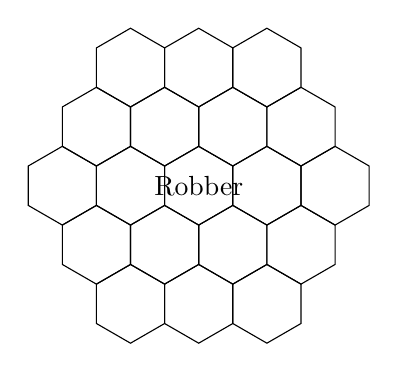
\begin{tikzpicture} [hexa/.style= {shape=regular polygon,regular polygon sides=6,minimum size=1cm, draw,inner sep=0,anchor=south,rotate=30}]
\foreach \j in {0,...,2}{%
\pgfmathsetmacro\end{2+\j} 
  \foreach \i in {0,...,\end}{%
  \node[hexa] (h\i;\j) at ({(\i-\j/2)*sin(60)},{\j*0.75}) {};}  }      
\node [circle,minimum size=1cm] at (h2;2) {Robber};
\foreach \j in {0,...,1}{%
  \pgfmathsetmacro\end{3-\j} 
  \foreach \i in {0,...,\end}{%
  \pgfmathtruncatemacro\k{\j+2}  
  \node[hexa] (h\i;\k) at ({(\i+\j/2-0.5)*sin(60)},{2.25+\j*0.75}) {};}  } 
\end{tikzpicture}
\end{center}

\begin{enumerate}[label=(\alph*)]
    \item Is this Markov chain irreducible? Is it aperiodic? \textbf{Answer:} $\boxed{\textnormal{Yes to both.}}$ The Markov chain is irreducible because it can get from anywhere to anywhere else. The Markov chain is  aperiodic because the robber can return back to a square in $2, 3, 4, 5, \dots$ moves, and the GCD of those numbers is $1$.
        \item What is the stationary distribution of this Markov chain? \textbf{Answer:} Since this is a random walk on an undirected graph, the stationary distribution is proportional to the degree sequence. The degree for the corner pieces is 3, the degree for the edge pieces is 4, and the degree for the center pieces is 6. To normalize this degree sequence, we divide by its sum. The sum of the degrees is $6(3) + 6(4) + 7(6) = 84$. Thus the stationary probability of being on a corner is $3/84 = 1/28$, on an edge is $4/84 =  1/21$, and in the center is $6/84 = 1/14$.
    \item What fraction of the time will the robber be in the center tile in this game, in the long run? \textbf{Answer:} By the above, $\boxed{1/14}$.
    \item What is the expected amount of moves it will take for the robber to return to the center tile? \textbf{Answer:} Since this chain is irreducible and aperiodic, to get the expected time to return we can just invert the stationary probability. Thus on average it will take $\boxed{14}$ turns for the robber to return to the center tile.
\end{enumerate}


\section{Problem-Solving Strategies} \smallskip \hrule height 2pt \smallskip

Contributions from Jessy Hwang, Yuan Jiang, Yuqi Hou
\begin{enumerate}
\item \textbf{Getting started.} Start by \emph{defining relevant events and random variables}. (``Let $A$ be the event that I pick the fair coin''; ``Let $X$ be the number of successes.'') Clear notion is important for clear thinking! Then decide what it is that you're supposed to be finding, in terms of your notation (``I want to find $P(X=3|A)$''). Think about what type of object your answer should be (a number? A random variable? A PMF? A PDF?) and what it should be in terms of.

\emph{Try simple and extreme cases}. To make an abstract experiment more concrete, try \emph{drawing a picture} or making up numbers that could have happened. Pattern recognition: does the structure of the problem resemble something we've seen before?
\item \textbf{Calculating probability of an event.} Use counting principles if the naive definition of probability applies. Is the probability of the complement easier to find? Look for symmetries. Look for something to condition on, then apply Bayes' Rule or the Law of Total Probability. 
\item \textbf{Finding the distribution of a random variable.} First make sure you need the full distribution not just the mean (see next item). Check the \emph{support} of the random variable: what values can it take on? Use this to rule out distributions that don't fit.  Is there a \emph{story} for one of the named distributions that fits the problem at hand?  Can you write the random variable as a function of an r.v. with a known distribution, say $Y = g(X)$?
\item \textbf{Calculating expectation.} If it has a named distribution, check out the table of distributions. If it's a function of an r.v. with a named distribution, try LOTUS. If it's a count of something, try breaking it up into indicator r.v.s. If you can condition on something natural, consider using Adam's law. 
\item \textbf{Calculating variance.} Consider independence, named distributions, and LOTUS. If it's a count of something, break it up into a sum of indicator r.v.s. If it's a sum, use properties of covariance. If you can condition on something natural, consider using Eve's Law.
\item \textbf{Calculating $E(X^2)$.}  Do you already know $E(X)$ or $\var(X)$? Recall that $\var(X) = E(X^2) - (E(X))^2$. Otherwise try LOTUS.
\item \textbf{Calculating covariance.} Use the properties of covariance. If you're trying to find the covariance between two components of a Multinomial distribution, $X_i, X_j$, then the covariance is $-np_ip_j$ for $i \neq j$.
\item \textbf{Symmetry.} If $X_1,\dots,X_n$ are i.i.d., consider using symmetry.
\item \textbf{Calculating probabilities of orderings.} Remember that all $n!$ ordering of i.i.d.~continuous random variables $X_1,\dots,X_n$ are equally likely.
\item \textbf{Determining independence.} There are several equivalent definitions. Think about simple and extreme cases to see if you can find a counterexample.
\item \textbf{Do a painful integral.} If your integral looks painful, see if you can write your integral in terms of a known PDF (like Gamma or Beta), and use the fact that PDFs integrate to $1$?
\item \textbf{Before moving on.} Check some simple and extreme cases, check whether the answer seems plausible, check for biohazards.\end{enumerate}


\section{Biohazards} \smallskip \hrule height 2pt \smallskip

Contributions from Jessy Hwang

\begin{enumerate} 
\item \textbf{Don't misuse the naive definition of probability.}   When answering ``What is the probability that in a group of 3 people, no two have the same birth month?'', it is \emph{not} correct to treat the people as indistinguishable balls being placed into 12 boxes, since that assumes the list of birth months \{January, January, January\} is just as likely as the list \{January, April, June\}, even though the latter is six times more likely. \\ 
\item \textbf{Don't confuse unconditional, conditional, and joint probabilities.}  In applying $P(A|B) = \frac{P(B|A)P(A)}{P(B)}$, it is \emph{not} correct to say ``$P(B) = 1$ because we know  $B$ happened''; $P(B)$ is the \emph{prior} probability of $B$. Don't confuse $P(A|B)$ with $P(A,B)$. \\
\item \textbf{Don't assume independence without justification.}  In the matching problem, the probability that card 1 is a match and card 2 is a match is not $1/n^2$.  Binomial and Hypergeometric are often confused; the trials are independent in the Binomial story and dependent in the Hypergeometric story. \\
\item \textbf{Don't forget to do sanity checks.} Probabilities must be between $0$ and $1$. Variances must be $\geq 0$. Supports must make sense. PMFs must sum to $1$. PDFs must integrate to $1$. \\
\item \textbf{Don't confuse random variables, numbers, and events.}  Let $X$ be an r.v. Then $g(X)$ is an r.v. for any function $g$. In particular, $X^2$, $|X|$, $F(X)$, and $I_{X>3}$ are r.v.s. $P(X^2 < X | X \geq 0), E(X), \var(X), $ and $g(E(X))$ are numbers. $X = 2$ and $F(X) \geq -1$ are events. It does not make sense to write $\int_{-\infty}^\infty F(X) dx$, because $F(X)$ is a random variable. It does not make sense to write $P(X)$, because $X$ is not an event. \\
\item \textbf{Don't confuse a random variable with its distribution.}  To get the PDF of $X^2$, you can't just square the PDF of $X$. The right way is to use transformations. To get the PDF of $X + Y$, you can't just add the PDF of $X$ and the PDF of $Y$. The right way is to compute the \hyperref[convolutions]{convolution}.
\item \textbf{Don't pull non-linear functions out of expectations.} $E(g(X))$ does not equal $g(E(X))$ in general. The St. Petersburg paradox is an extreme example.  See also Jensen's inequality. The right way to find $E(g(X))$ is with \hyperref[lotus]{LOTUS}.
\end{enumerate}

\vspace{1.5in}

\section{Distributions in R} \smallskip \hrule height 2pt \smallskip

\bigskip

\begin{center}
\begin{tabular}{cc}
\hline
\textbf{Command} & \textbf{What it does} \\
\hline
\texttt{help(distributions)} & shows documentation on distributions\\
\texttt{dbinom(k,n,p)} & PMF $P(X=k)$ for $X \sim \Bin(n,p)$\\
\texttt{pbinom(x,n,p)} & CDF $P(X \leq x)$ for $X \sim \Bin(n,p)$\\
\texttt{qbinom(a,n,p)} &   $a$th quantile for $X \sim \Bin(n,p)$\\
\texttt{rbinom(r,n,p)} &  vector of $r$ i.i.d.~$\Bin(n,p)$ r.v.s\\
\texttt{dgeom(k,p)} & PMF $P(X=k)$ for $X \sim \Geom(p)$\\
\texttt{dhyper(k,w,b,n)} & PMF $P(X=k)$ for $X \sim \HGeom(w,b,n)$\\
\texttt{dnbinom(k,r,p)} & PMF $P(X=k)$ for $X \sim \NBin(r,p)$\\
\texttt{dpois(k,r)} & PMF $P(X=k)$ for $X \sim \Pois(r)$\\
\texttt{dbeta(x,a,b)} & PDF $f(x)$ for $X \sim \Beta(a,b)$\\
\texttt{dchisq(x,n)} & PDF $f(x)$ for $X \sim \chi^2_n$\\
\texttt{dexp(x,b)} & PDF $f(x)$ for $X \sim \Expo(b)$\\
\texttt{dgamma(x,a,r)} & PDF $f(x)$ for $X \sim \Gam(a,r)$\\
\texttt{dlnorm(x,m,s)} & PDF $f(x)$ for $X \sim \mathcal{LN}(m,s^2)$\\
\texttt{dnorm(x,m,s)} & PDF $f(x)$ for $X \sim \N(m,s^2)$\\
\texttt{dt(x,n)} & PDF $f(x)$ for $X \sim t_n$\\
\texttt{dunif(x,a,b)} & PDF $f(x)$ for $X \sim \Unif(a,b)$\\
\hline
\end{tabular}
\end{center}

The table above gives R commands for working with various named distributions. Commands analogous to \texttt{pbinom}, \texttt{qbinom}, and \texttt{rbinom} work for the other distributions in the table. For example, \texttt{pnorm}, \texttt{qnorm}, and \texttt{rnorm} can be used to get the CDF,  quantiles, and random generation for the Normal.  For the Multinomial, \texttt{dmultinom} can be used for calculating the joint PMF and \texttt{rmultinom} can be used for generating random vectors. For the Multivariate Normal, after installing and loading the \texttt{mvtnorm} package \texttt{dmvnorm} can be used for calculating the joint PDF and \texttt{rmvnorm} can be used for generating random vectors.

\vspace{4in}


\section{Recommended Resources} \smallskip \hrule height 2pt \smallskip

\bigskip

\begin{itemize}
\item Introduction to Probability Book (\url{http://bit.ly/introprobability})
\item Stat 110 Online (\url{http://stat110.net})
\item Stat 110 Quora Blog (\url{https://stat110.quora.com/})
\item Quora Probability FAQ (\url{http://bit.ly/probabilityfaq})
\item R Studio (\url{https://www.rstudio.com})
\item LaTeX File (\texttt{\href{https://github.com/wzchen/probability_cheatsheet}{github.com/wzchen/probability\_cheatsheet}})
\end{itemize}

\begin{center}\emph{Please share this cheatsheet with friends!} \url{http://wzchen.com/probability-cheatsheet}\end{center}

\end{multicols*}

\section{Table of Distributions} 


\begin{center}
\renewcommand{\arraystretch}{3.7}
\begin{tabular}{cccccc}
\textbf{Distribution} & \textbf{PMF/PDF and Support} & \textbf{Expected Value}  & \textbf{Variance} & \textbf{MGF}\\
\hline 
\shortstack{Bernoulli \\ \Bern($p$)} & \shortstack{$P(X=1) = p$ \\$ P(X=0) = q=1-p$} & $p$ & $pq$ & $q + pe^t$ \\
\hline
\shortstack{Binomial \\ \Bin($n, p$)} & \shortstack{$P(X=k) = {n \choose k}p^k q^{n-k}$  \\ $k \in \{0, 1, 2, \dots n\}$}& $np$ & $npq$ & $(q + pe^t)^n$ \\
\hline
\shortstack{Geometric \\ \Geom($p$)} & \shortstack{$P(X=k) = q^kp$  \\ $k \in \{$0, 1, 2, \dots $\}$}& $q/p$ & $q/p^2$ & $\frac{p}{1-qe^t}, \, qe^t < 1$\\
\hline
\shortstack{Negative Binomial \\ \NBin($r, p$)} & \shortstack{$P(X=n) = {r + n - 1 \choose r -1}p^rq^n$ \\ $n \in \{$0, 1, 2, \dots $\}$} & $rq/p$ & $rq/p^2$ &  $(\frac{p}{1-qe^t})^r, \, qe^t < 1$\\
\hline
\shortstack{Hypergeometric \\ \Hypergeometric($w, b, n$)} & \shortstack{$P(X=k) = \sfrac{{w \choose k}{b \choose n-k}}{{w + b \choose n}}$ \\ $k \in \{0, 1, 2, \dots,  n\}$} & $\mu = \frac{nw}{b+w}$ &$\left(\frac{w+b-n}{w+b-1} \right) n\frac{\mu}{n}(1 - \frac{\mu}{n})$& messy  \\
\hline
\shortstack{Poisson \\ \Pois($\lambda$)} & \shortstack{$P(X=k) = \frac{e^{-\lambda}\lambda^k}{k!}$ \\ $k \in \{$0, 1, 2, \dots $\}$} & $\lambda$ & $\lambda$ & $e^{\lambda(e^t-1)}$ \\
\hline
\hline
\shortstack{Uniform \\ \Unif($a, b$)} & \shortstack{$ f(x) = \frac{1}{b-a}$ \\$ x \in (a, b) $} & $\frac{a+b}{2}$ & $\frac{(b-a)^2}{12}$ &  $\frac{e^{tb}-e^{ta}}{t(b-a)}$\\
\hline
\shortstack{Normal \\ $\N(\mu, \sigma^2)$} & \shortstack{$f(x) = \frac{1}{\sigma \sqrt{2\pi}} e^{-\sfrac{(x - \mu)^2}{(2 \sigma^2)}}$ \\ $x \in (-\infty, \infty)$} & $\mu$  & $\sigma^2$ & $e^{t\mu + \frac{\sigma^2t^2}{2}}$\\
\hline
\shortstack{Exponential \\ $\Expo(\lambda)$} & \shortstack{$f(x) = \lambda e^{-\lambda x}$\\$ x \in (0, \infty)$} & $\frac{1}{\lambda}$  & $\frac{1}{\lambda^2}$ & $\frac{\lambda}{\lambda - t}, \, t < \lambda$\\
\hline
\shortstack{Gamma \\ $\Gam(a, \lambda)$} & \shortstack{$f(x) = \frac{1}{\Gamma(a)}(\lambda x)^ae^{-\lambda x}\frac{1}{x}$\\$ x \in (0, \infty)$} & $\frac{a}{\lambda}$  & $\frac{a}{\lambda^2}$ & $\left(\frac{\lambda}{\lambda - t}\right)^a, \, t < \lambda$\\
\hline
\shortstack{Beta \\ \Beta($a, b$)} & \shortstack{$f(x) = \frac{\Gamma(a+b)}{\Gamma(a)\Gamma(b)}x^{a-1}(1-x)^{b-1}$\\$x \in (0, 1) $} & $\mu = \frac{a}{a + b}$  & $\frac{\mu(1-\mu)}{(a + b + 1)}$ & messy \\
\hline
\shortstack{Log-Normal \\ $\mathcal{LN}(\mu,\sigma^2)$} & \shortstack{$\frac{1}{x\sigma \sqrt{2\pi}}e^{-(\log x - \mu)^2/(2\sigma^2)}$\\$x \in (0, \infty)$} & $\theta = e^{ \mu + \sigma^2/2}$ & $\theta^2 (e^{\sigma^2} - 1)$ & doesn't exist\\
\hline
\shortstack{Chi-Square \\ $\chi_n^2$} & \shortstack{$\frac{1}{2^{n/2}\Gamma(n/2)}x^{n/2 - 1}e^{-x/2}$\\$x \in (0, \infty) $} & $n$  & $2n$ & $(1 - 2t)^{-n/2}, \, t < 1/2$\\
\hline
\shortstack{Student-$t$ \\ $t_n$} & \shortstack{$\frac{\Gamma((n+1)/2)}{\sqrt{n\pi} \Gamma(n/2)} (1+x^2/n)^{-(n+1)/2}$\\$x \in (-\infty, \infty)$} & $0$ if $n>1$ & $\frac{n}{n-2}$ if $n>2$ & doesn't exist\\
\hline
\end{tabular}
\end{center}


\end{document}